 \documentclass[11pt]{article}
\usepackage{pdfpages}

% Change "review" to "final" to generate the final (sometimes called camera-ready) version.
% Change to "preprint" to generate a non-anonymous version with page numbers.
\usepackage[preprint]{acl}

% Standard package includes
\usepackage{times}
\usepackage{latexsym}
\usepackage{supertabular} 
\usepackage{booktabs}
\usepackage{amsfonts,amsmath,amssymb,amsthm}
\usepackage{multirow}
\usepackage{booktabs}
\usepackage[table]{xcolor}
\usepackage{graphicx}
\usepackage{adjustbox}
\usepackage{amsfonts}
\usepackage{amssymb}
\usepackage{colortbl}
\usepackage{svg}
% For proper rendering and hyphenation of words containing Latin characters (including in bib files)
\usepackage[T1]{fontenc}
\usepackage{url}
% For Vietnamese characters
% \usepackage[T5]{fontenc}
% See https://www.latex-project.org/help/documentation/encguide.pdf for other character sets

% This assumes your files are encoded as UTF8
\usepackage[utf8]{inputenc}

% This is not strictly necessary, and may be commented out,
% but it will improve the layout of the manuscript,
% and will typically save some space.
\usepackage{microtype}

% This is also not strictly necessary, and may be commented out.
% However, it will improve the aesthetics of text in
% the typewriter font.
\usepackage{inconsolata}

%Including images in your LaTeX document requires adding
%additional package(s)
\usepackage{graphicx}
\usepackage{fontawesome5}

% If the title and author information does not fit in the area allocated, uncomment the following
%
%\setlength\titlebox{<dim>}
%
% and set <dim> to something 5cm or larger.

\title{The Necessity of Setting Temperature in LLM-as-a-Judge}

% Author information can be set in various styles:
% For several authors from the same institution:
% \author{Author 1 \and ... \and Author n \\
%         Address line \\ ... \\ Address line}
% if the names do not fit well on one line use
%         Author 1 \\ {\bf Author 2} \\ ... \\ {\bf Author n} \\
% For authors from different institutions:
% \author{Author 1 \\ Address line \\  ... \\ Address line
%         \And  ... \And
%         Author n \\ Address line \\ ... \\ Address line}
% To start a separate ``row'' of authors use \AND, as in
% \author{Author 1 \\ Address line \\  ... \\ Address line
%         \AND
%         Author 2 \\ Address line \\ ... \\ Address line \And
%         Author 3 \\ Address line \\ ... \\ Address line}

\author{
 \textbf{Lujun Li\textsuperscript{$\spadesuit$1}},
 \textbf{Lama Sleem\textsuperscript{$\spadesuit$1}},
 \textbf{Yangjie Xu\textsuperscript{$\spadesuit$1}},
 \\
 \textbf{Yewei Song\textsuperscript{1}},
  \textbf{Aolin Jia\textsuperscript{2}},
 \textbf{Jerome Francois\textsuperscript{1}},
 \textbf{Radu State\textsuperscript{1}},
\\
 \textsuperscript{1}University of Luxembourg,
 \textsuperscript{2}ETH Zürich
\\
 % \small{
 %   \textbf{Correspondence:} \href{mailto:lujun.li@uni.lu}{lujun.li@uni.lu}
 % }
}

%  Lujun Li, Lama Sleem，Yangjie Xu, Yiqun Wang, Yewei Song, Aolin Jia, Radu State

%\author{
%  \textbf{First Author\textsuperscript{1}},
%  \textbf{Second Author\textsuperscript{1,2}},
%  \textbf{Third T. Author\textsuperscript{1}},
%  \textbf{Fourth Author\textsuperscript{1}},
%\\
%  \textbf{Fifth Author\textsuperscript{1,2}},
%  \textbf{Sixth Author\textsuperscript{1}},
%  \textbf{Seventh Author\textsuperscript{1}},
%  \textbf{Eighth Author \textsuperscript{1,2,3,4}},
%\\
%  \textbf{Ninth Author\textsuperscript{1}},
%  \textbf{Tenth Author\textsuperscript{1}},
%  \textbf{Eleventh E. Author\textsuperscript{1,2,3,4,5}},
%  \textbf{Twelfth Author\textsuperscript{1}},
%\\
%  \textbf{Thirteenth Author\textsuperscript{3}},
%  \textbf{Fourteenth F. Author\textsuperscript{2,4}},
%  \textbf{Fifteenth Author\textsuperscript{1}},
%  \textbf{Sixteenth Author\textsuperscript{1}},
%\\
%  \textbf{Seventeenth S. Author\textsuperscript{4,5}},
%  \textbf{Eighteenth Author\textsuperscript{3,4}},
%  \textbf{Nineteenth N. Author\textsuperscript{2,5}},
%  \textbf{Twentieth Author\textsuperscript{1}}
%\\
%\\
%  \textsuperscript{1}Affiliation 1,
%  \textsuperscript{2}Affiliation 2,
%  \textsuperscript{3}Affiliation 3,
%  \textsuperscript{4}Affiliation 4,
%  \textsuperscript{5}Affiliation 5
%\\
%  \small{
%    \textbf{Correspondence:} \href{mailto:email@domain}{email@domain}
%  }

%}

\usepackage{times}
\usepackage{latexsym}
\usepackage[T1]{fontenc}
\usepackage{inconsolata}
\usepackage{tcolorbox}
\tcbuselibrary{skins,breakable,xparse}

\newtcolorbox{promptbox}[2][]{
  enhanced,
  breakable,
  colback=gray!10,
  colframe=gray!70,
  coltitle=white,
  fonttitle=\bfseries\small\ttfamily\color{white},
  fontupper=\ttfamily\footnotesize,
  boxrule=0.8pt,
  title={#2},
  title style={fill=gray!70},
  left=5mm, right=5mm,
  top=3mm, bottom=3mm,
  arc=2mm,
  borderline west={3pt}{0pt}{gray!80},
  boxsep=2pt,
  #1
}

\newtcolorbox{userbox}[2][]{
  enhanced,
  breakable,
  colback=blue!3,
  colframe=blue!60!black,
  coltitle=white,
  fonttitle=\bfseries\small\ttfamily\color{white},
  fontupper=\ttfamily\footnotesize,
  boxrule=0.8pt,
  title={#2},
  title style={fill=blue!60!black},
  left=5mm, right=5mm,
  top=3mm, bottom=3mm,
  arc=2mm,
  borderline west={3pt}{0pt}{blue!70},
  boxsep=2pt,
  #1
}


\newtcolorbox{responsebox}[2][]{
  enhanced,
  breakable,
  colback=green!5,
  colframe=green!65!black,
  coltitle=white,
  fonttitle=\bfseries\small\ttfamily\color{white},
  fontupper=\ttfamily\footnotesize,
  boxrule=0.8pt,
  title={#2},
  title style={fill=green!65!black},
  left=5mm, right=5mm,
  top=3mm, bottom=3mm,
  arc=2mm,
  borderline west={3pt}{0pt}{green!75},
  boxsep=2pt,
  #1
}


\definecolor{lightblue}{RGB}{230,240,255}
\definecolor{lightred}{RGB}{255,230,230}

\begin{document}
 \maketitle
\begin{abstract}
% \def\thefootnote{$\spadesuit$}\footnotetext{These authors contributed equally to this work.}\def\thefootnote{\arabic{footnote}}

% LLM-as-a-Judge has emerged as an effective and low-cost paradigm for evaluating text quality and factual correctness. Prior studies have shown substantial agreement between LLM judges and human experts, even on tasks that are difficult to assess automatically. In practice, researchers commonly employ 
% fixed temperature configurations during the evaluation process — with values 
% of 0.1 and 1.0 being the most prevalent choices — a convention that is largely 
% empirical rather than principled. However, recent researches suggest that LLM 
% performance exhibits non-trivial sensitivity to temperature settings, that 
% lower temperatures do not universally yield optimal outcomes, and that such 
% effects are highly task-dependent. This raises a critical research question: 
% \textit{does temperature influence judge performance in LLM-centric evaluation?} 
% To address this, we systematically investigate the relationship between 
% temperature and judge performance through a series of controlled experiments, 
% and further adopt a causal inference framework within our empirical statistical 
% analysis to rigorously examine the direct causal effect of temperature on judge 
% behavior, offering actionable engineering insights for the design of 
% LLM-centric evaluation pipelines.
Using large language models (LLMs) as judges for evaluating model outputs has emerged as an important paradigm for automated evaluation. However, the choice of decoding temperature in LLM-as-a-Judge settings is still largely chosen empirically, with limited systematic evidence on its impact. To address this gap, we conduct a systematic study of how temperature affects judgment behavior across different LLM judge models, prompting strategies, and evaluation paradigms. Our results show that higher temperatures generally decrease judgment consistency and increase formatting errors, while also exposing latent uncertainty that tends to remain suppressed under low-temperature decoding, particularly in ambiguous cases. Further analysis suggests that higher temperatures can serve as an exploratory mechanism and may improve judging performance in complex or uncertain evaluation scenarios. Overall, low-temperature settings are better suited to tasks that prioritize stability and reproducibility, whereas higher-temperature settings are more appropriate for scenarios involving substantial ambiguity or complexity, where exploration of the judge’s decision space is beneficial. These findings suggest that, in LLM-as-a-Judge systems, temperature should be treated not as a fixed hyperparameter, but as a controllable, task-dependent design choice that mediates the trade-off between reliability and exploration.
\end{abstract}


% \footnote{Code available at: \url{https://anonymous.4open.science/r/LLMJudgeTempCausal-67F9}}


\section{Introduction}

With the widespread adoption of large language models (LLMs) in domains such as text generation, question-answering systems, and automated evaluation, assessing the output quality of LLMs has emerged as a pivotal challenge \cite{gu2025surveyllmasajudge}. Recent trends indicate that employing LLMs as evaluators or judges---commonly termed \textbf{LLM-as-a-Judge}---is progressively supplanting common human-annotated evaluation. This shift is driven by the capacity of model-based evaluation to substantially reduce human labeling costs, accelerate assessment cycles, and demonstrate superior consistency in sophisticated tasks like multi-turn dialogues and open-ended question answering \cite{tang2025learning}. Nevertheless, existing research reveals that LLM-based evaluation outcomes are susceptible to influences from generation parameters, such as \textbf{sampling temperature}~\cite{du2025optimizingtemperaturelanguagemodels}, which can induce score volatility, positional bias and decreased consistency, thus undermining the interpretability and reliability of the assessments.


\begin{figure}[htbp]
  \centering
    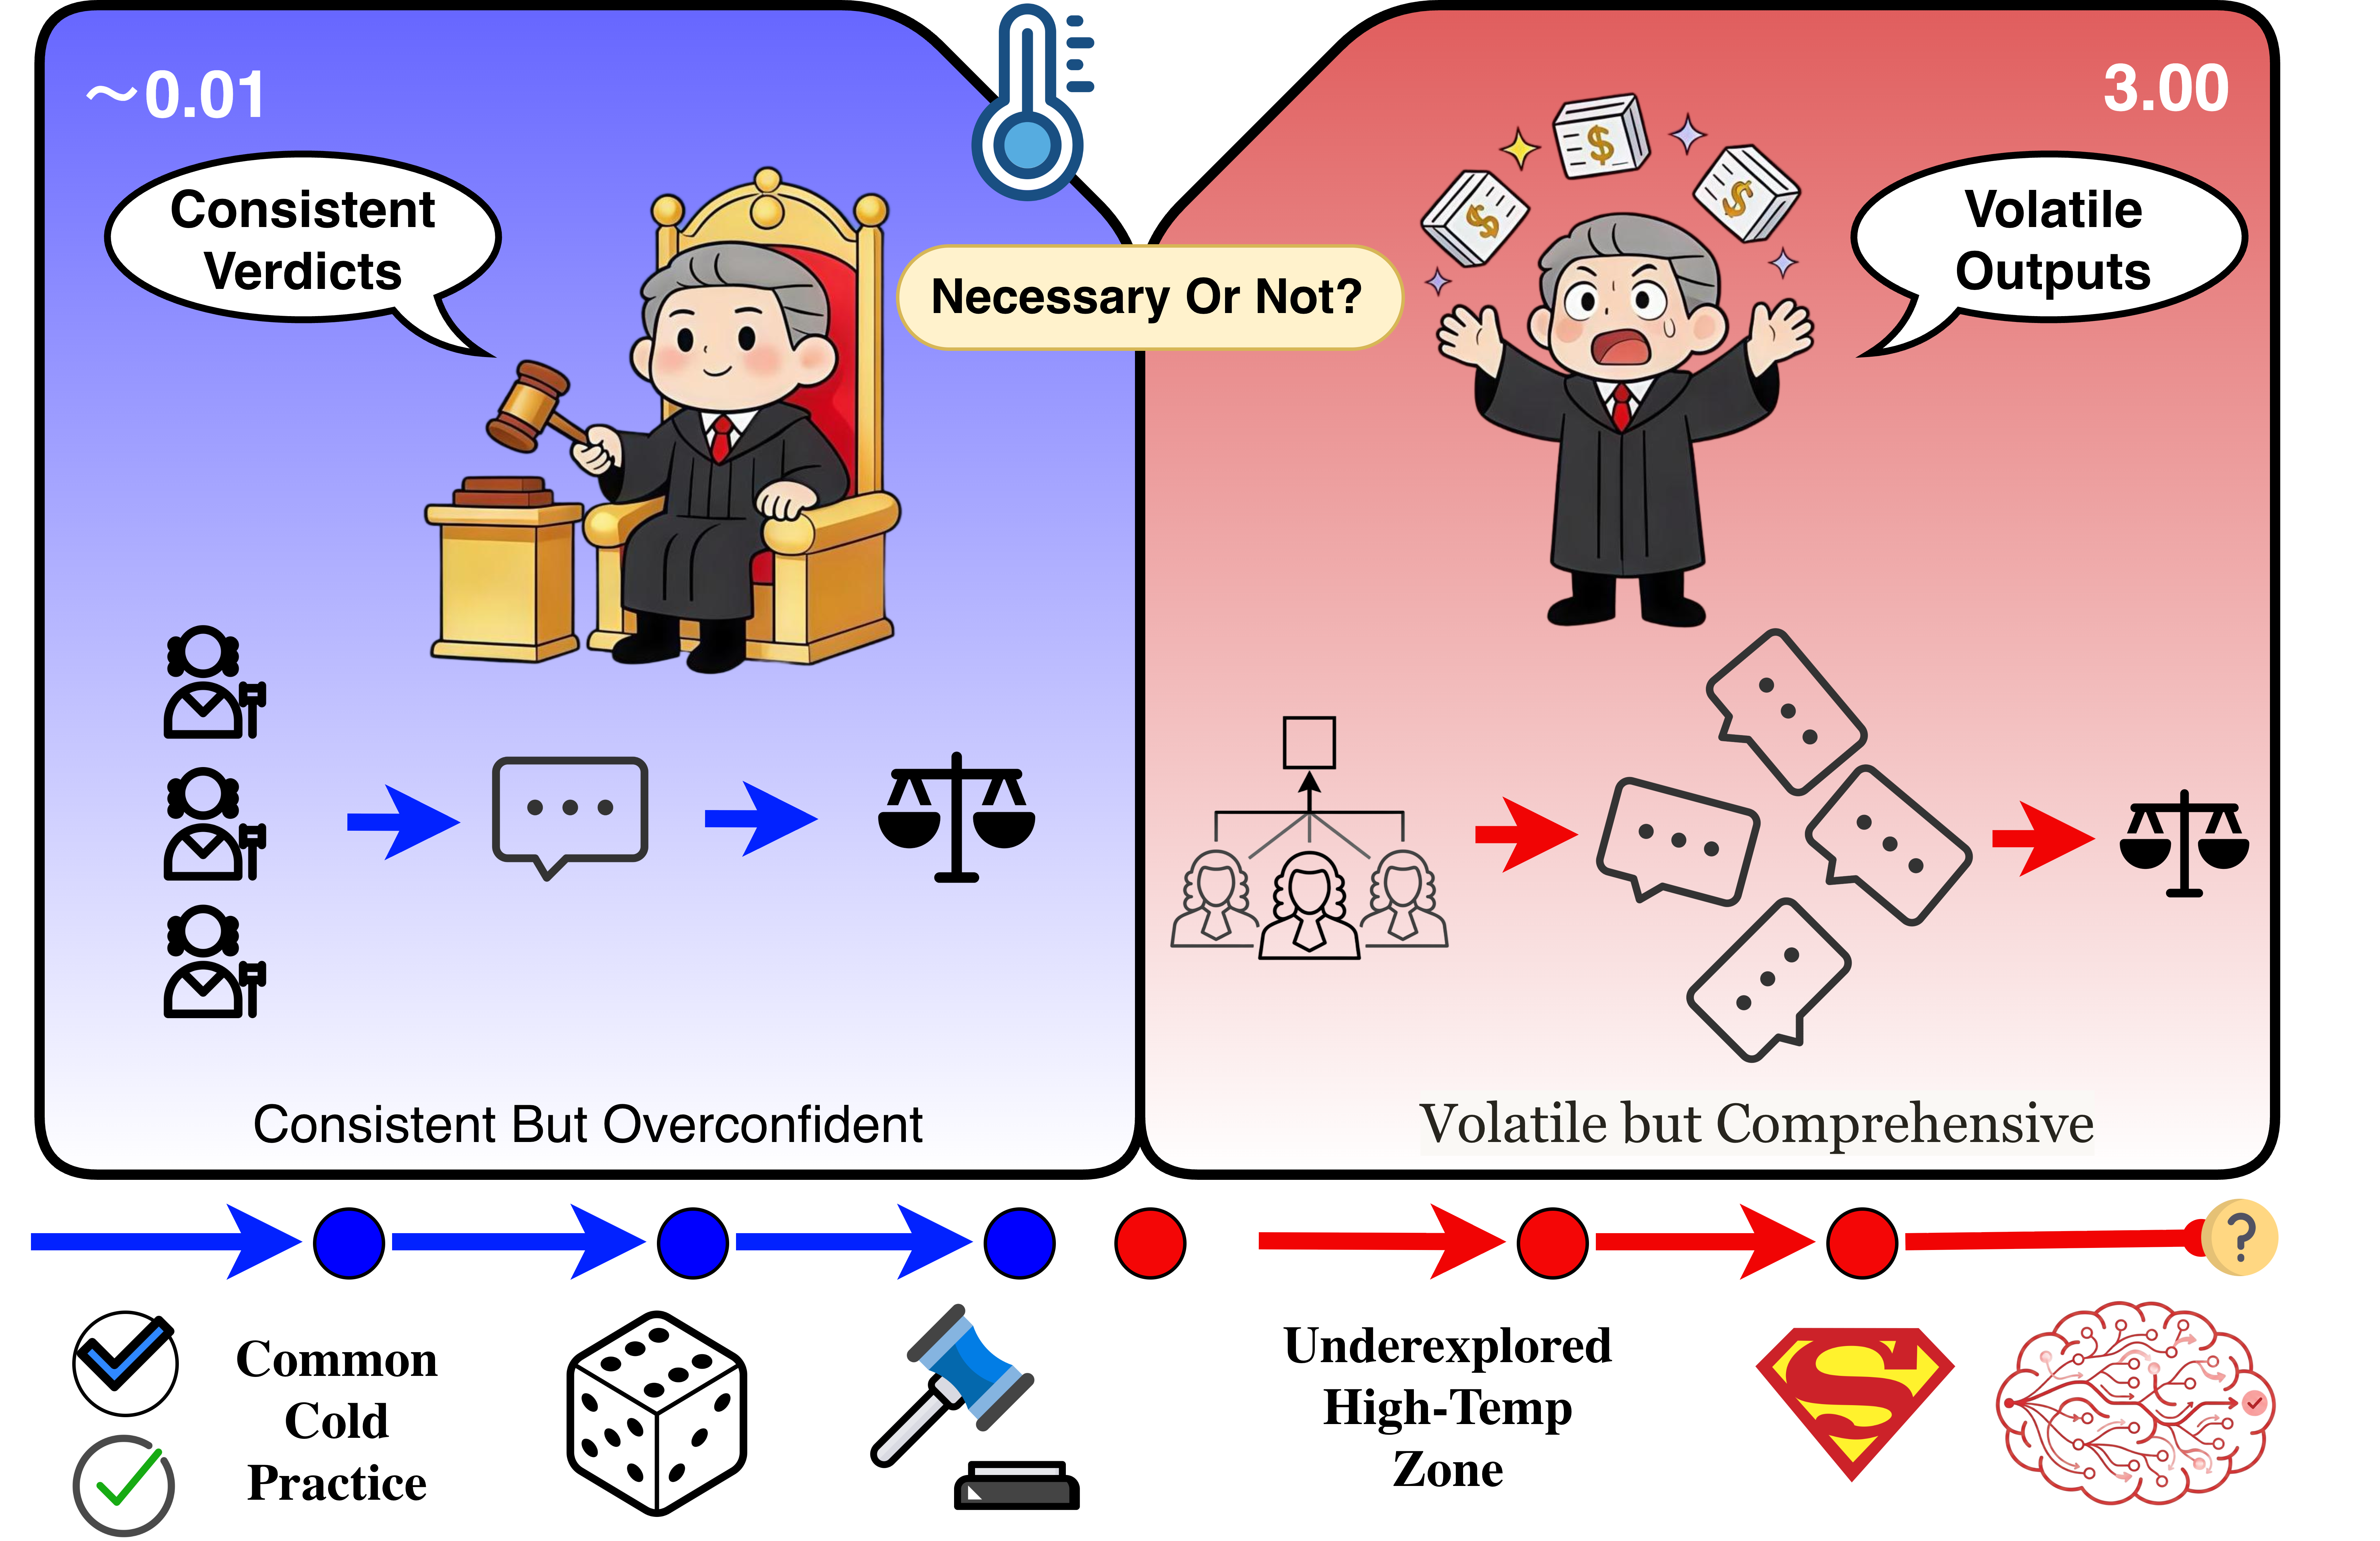
\includegraphics[width=\linewidth]{photos/temperature_LLM_Judge.drawio.png}
  \caption{LLM-as-a-Judge Paradigm}
  \label{fig:llmasaaj}
\end{figure}


To the best of our knowledge, empirical settings for the LLM temperature---such as values close to 0---are commonly employed in LLM-as-a-Judge paradigms. This practice is well-understood, particularly given cost considerations and reproducibility, as more powerful models have been demonstrated to exhibit exceptionally high alignment with human judgments \cite{10.5555/3666122.3668142}. However, a critical question remains: \textbf{Does the temperature setting influence the evaluative performance of LLM judges, and is it necessary to configure different temperatures for evaluation?} Moreover, the extent to which different LLM-as-a-judge configurations are affected represents a still underexplored avenue in real-world applications senarios. Therefore, although the role of temperature control in the diversity of generation \cite{peeperkorn2024temperaturecreativityparameterlarge} has been extensively investigated, its underlying mechanisms on the \textbf{``judging behavior''} remain underexplored through a systematic analysis. 

This work makes three main contributions. \textbf{First}, we conduct an large-scale empirical investigation using two datasets and multiple state-of-the-art open-source models to examine the effects of temperature. We perform more than one million evaluation runs across diverse temperature configurations, including varied prompting strategies, multiple LLM architectures, and different judging paradigms. The results provide robust statistical evidence and practical insights, demonstrating that decoding temperature is a key control knob that strongly affects stability, format compliance, and reproducibility. \textbf{Second}, we present a case study analyzing the outputs of LLM judges, revealing noteworthy insights into their behavioral dynamics under different settings. \textbf{Third}, we further investigate how higher temperatures can improve judge performance by evaluating Ensemble Thermo-Judge on a set of ambiguous cases, thereby validating the value of leveraging diverse temperature settings for building a well-rounded judge.

\section{Related work}

\noindent \textbf{Commonly used but understudied:} Although LLMs have different types of bias \cite{ye2024justiceprejudicequantifyingbiases,shi-etal-2025-judging,chen-etal-2024-humans}, LLMs-as-a-Judge have emerged as a novel form of annotator capable of performing classification tasks across diverse text-related domains~\cite{GU2026101253}. \textbf{Temperature settings have already been widely adopted} in LLM-as-a-Judge frameworks, with substantial variation across cases, typically ranging from 0.01 to 1.0. Fundamentally, they remain deep learning classifiers, with their in-context learning generalization enabling evaluations tailored to varied requirements. \citeauthor{10.5555/3666122.3668142} validated the high alignment between LLMs-as-a-Judge and human judgments through extensive manual inspections and experiments across multiple dimensions, employing a fixed temperature setting of 0.7. \citeauthor{shi-etal-2025-judging} conducted an in-depth investigation into position bias under diverse configurations by introducing metrics such as repeated stability and position consistency, underscoring the necessity of swapping candidate pair positions; however, this study only adopted a single temperature of 1.0. Another work~\cite{wei2025systematicevaluationllmasajudgellm} preliminarily examined the impact of temperature on LLMs-as-a-Judge, testing values from 0.0 to 0.7 and finding peak self-consistency and accuracy at 0.1; nevertheless, the overall temperature effects were not pronounced, the range was limited, and the exploration remained insufficiently comprehensive. 



\noindent \textbf{T affects Judging:}  However, \citeauthor{LI2025242} provides preliminary evidence that higher temperature settings can affect LLM outputs and may even improve performance in some cases. Related studies further suggest that temperature can substantially influence the behavior of LLMs \cite{renze-2024-effect, deepseek_api_temp_2026}, raising the possibility that it may also affect the effectiveness of LLM-as-a-Judge systems. However, prior explorations of temperature effects remain limited in both breadth and depth and whether distinct temperature settings are required for LLM-as-a-Judge systems to optimize judgment outcomes remains an open question.



\section{Methods}

\subsection{Definition}

Let \( v \in \mathcal{V} \) denote the final verdict in the discrete verdict space \( \mathcal{V} \) \cite{ACKLEY1985147}.
Given a question \( q \), we consider an input tuple \( (x, r) \), where \( x \) denotes the model-generated answer to \( q \), and \( r \) denotes the reference (gold) answer when available. In settings without reference answers, the judgment is performed solely based on \( x \).

\begin{equation}
\begin{aligned}
p_T(v = i \mid x, r)
&= \frac{\exp\!\left(a_i(x, r)/T\right)}
{\sum_{j \in \mathcal{V}} \exp\!\left(a_j(x, r)/T\right)}, \\
\hat{v}
&= \mathrm{Decode}\!\left(p_T(\cdot \mid x, r)\right).
\end{aligned}
\end{equation}

Here, \( a_i(x, r) \) denotes the logit associated with verdict \( i \), and \( T > 0 \) is the decoding temperature. When the reference answer \( r \) is not available, the formulation naturally reduces to conditioning on \( x \) alone. The temperature rescales the logits to control the sharpness of the verdict distribution without altering their relative order, and therefore does not change the ranking of candidate output tokens. In practice, this implies that temperature primarily affects decision variance and reproducibility, rather than inducing substantial shifts in average accuracy. Furthermore, due to the autoregressive nature of decoding, LLMs generation typically adhere to a Markovian inference process\cite{zhang2026markovcategoricalframeworklanguage}, with output diversity governed by a random seed 
that controls the initial generation; however, incorporating an initial reasoning 
phase—such as Chain-of-Thought (CoT) prompting \citep{DBLP:journals/corr/abs-2201-11903}—can lead to fundamentally divergent 
model outputs.





% Under a randomized or otherwise identified design, we estimate a causal regression model in which the judge outcome \(Y_i\) is expressed as a function of temperature \(T_i\), prompt template \(P_i\), and judge model \(L_i\). In this specification, \(T_i\) is the focal treatment, while \(P_i\) and \(L_i\) are pre-treatment contextual factors that may moderate the causal effect of temperature. Accordingly, the interaction terms \(P_i \times T_i\) and \(L_i \times T_i\) are included to assess treatment effect heterogeneity across prompt templates and judge models. We further include the three-way interaction \(P_i \times L_i \times T_i\) as a hypothesis-driven term to test whether the heterogeneity of the temperature effect jointly depends on prompt template and judge model. To preserve the hierarchical modeling principle, all associated lower-order interactions and main effects are retained in the specification.

% To preserve the hierarchical modeling principle, all lower-order main effects and two-way interactions associated with the three-way interaction are retained in the specification. This ensures that the higher-order term is interpreted relative to a properly specified lower-order structure and avoids an under-hierarchical formulation of interaction effects. Accordingly, the model is written as follows:

% Under a randomized or otherwise identified design, we estimate a causal regression model in which the judge outcome $Y_i$ depends on temperature $T_i$, prompt template $P_i$, and judge model $L_i$. The main treatment is $T_i$, while $P_i$ and $L_i$ are pre-treatment factors that may moderate its effect. We therefore include the interactions $P_i \times T_i$ and $L_i \times T_i$ to assess heterogeneity across prompt templates and judge models, as well as the three-way interaction $P_i \times L_i \times T_i$ to test whether this heterogeneity jointly depends on both factors. To follow the hierarchical modeling principle, all related main effects and lower-order interactions are retained. The model is specified as follows:



% \begin{equation}
%     \begin{split}
%     Y_i =\;& \beta_0 + \beta_1 T_i + \beta_2 P_i + \beta_3 L_i \\
%     &+ \beta_4 (P_i \times T_i)
%     + \beta_5 (L_i \times T_i)
%     + \beta_6 (P_i \times L_i) \\
%     &+ \beta_7 (P_i \times L_i \times T_i)
%     + \varepsilon_i .
%     \end{split}
% \end{equation}


% This model is designed to identify the causal effect of temperature, as well as heterogeneity in that effect across $P_i$ and $L_i$, rather than the full causal effects of $P_i$ and $L_i$ themselves.








% \begin{figure}[!htbp]
%   \centering
%   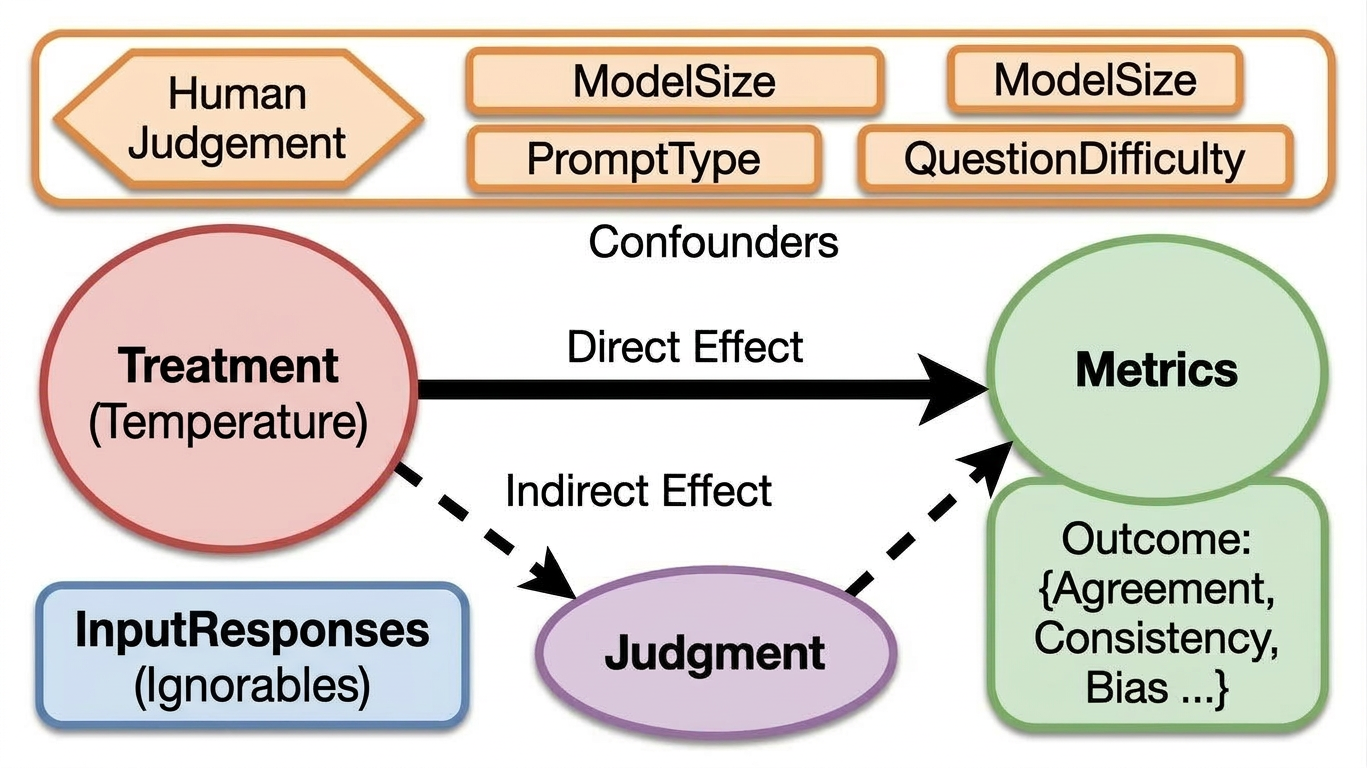
\includegraphics[width=0.95\linewidth]{photos/DAGs.png}
%   \caption{DAGs}
%   \label{fig:dags}
% \end{figure}


\subsection{Experimental Design}

In this study, we examine six temperature settings: \([0.01, 0.5, 1.0, 1.5, 2.0, 3.0]\). 
To reduce stochastic variability, each experimental condition is repeated ten times using different random seeds. We employ \texttt{Qwen/Qwen3-Next-80B-A3B-Instruct-FP8}~\cite{qwen2.5-1m, qwen3technicalreport} and \texttt{google/gemma-3-27b-it}~\cite{gemma_2025} as the primary open-weight judge models, supplemented with additional models for robustness checks and auxiliary analyses, to assess whether temperature-induced effects generalize across models. The temperature range follows prior work~\cite{LI2025242}, which also reports that \texttt{top\_p} and \texttt{top\_k} have limited effects on LLMs' capabilities. Accordingly, we fix \texttt{top\_p} at 0.95 and the maximum generation length at 2048 tokens in all experiments.

Following the taxonomy of judge types proposed by \cite{10.5555/3666122.3668142}, we examine three representative LLM-as-a-Judge paradigms: \textbf{pairwise comparison}, \textbf{single-answer grading}, and \textbf{reference-guided grading}. Pairwise comparison requires the model to select the better response between two candidates; single-answer grading assigns an absolute score or label to a single response; and reference-guided grading evaluates a response with respect to a provided gold answer (see prompt details in Appendix~\ref{appendix:prompt template}). Each paradigm is tested using both the direct base prompt and the CoT prompt, as these represent the most common approaches in LLM-as-a-judge evaluations. 
We do not additionally test few-shot prompting here, primarily due to its potential to introduce unclear biases whose interpretability remains underexplored. 
Furthermore, while positional bias (i.e., LLM preferences when options are presented first versus last) is a compelling topic, it is excluded from this study, as our primary focus is the impact of temperature on the judge performance. In addition, we conduct supplementary experiments on a new ensemble judge method to demonstrate the complementary role of higher temperatures in certain scenarios.







\subsection{Dataset}

For our dataset selection, we primarily employ \textbf{MT-Bench Human Judgments} \cite{10.5555/3666122.3668142}, which encompasses extensive data from models such as GPT-3.5-Turbo, Vicuna-13B-v1.2, Llama-13B, and others, all derived from the MT-Bench dataset~\cite{10.5555/3666122.3668142}. Its main advantage lies in the inclusion of \textbf{human-verified annotations}, which allow us to assess the alignment between LLM-as-a-Judge performance and human evaluators under different temperature settings. From this dataset, we randomly sampled 350 questions to construct our temperature test set.

Since MT-Bench was released in late 2023, we supplement with \textbf{MMLU-Pro}~\cite{10.5555/3737916.3740934}, which offers substantially greater difficulty compared to the original MMLU and recommends CoT reasoning for all tasks. This makes it particularly suitable for assessing LLM-as-a-Judge performance on complex reasoning outcomes. Here, we sample 150 items from the original test set according to the category proportions of the dataset, and then randomly select three open-source models---meta-llama/Llama-3.1-8B-Instruct, google/gemma-3-12b-it, and Qwen/Qwen2.5-14B-Instruct---to generate their responses for being judged. However, since this dataset lacks human annotations, we employed the current SOTA (as of February 2026) GPT-5.4 as the replacement to partially substitute for human-verified annotations (see prompt details in Appendix~\ref{appendix:judge_prompt_4.5}). Therefore, our open-source dataset comprises 500 questions, responses, and human judge selections (with partial coverage), enabling us to systematically investigate the impact of temperature on LLM-as-a-Judge performance.










\subsection{Metrics}

Three metrics are used to evaluate the judge behavior: agreement rate, consistency, and error rate. 
\textbf{Agreement Rate (AGR)} measures the extent to which the decisions produced by the LLM judge align with human-verified reference labels (i.e., consistency with the decision made by the ``judge in the court''), and thus serves as a primary indicator of judge performance.
$$
\text{AGR} = \frac{1}{N}\sum_{i=1}^N \mathbf{1}(\hat{y}_i = y_i^*) \cdot \mathbf{1}(\hat{y}_i \neq \emptyset \wedge y_i^* \neq \emptyset)
$$
where $\hat{y}_i\in\{\text{model\_a, model\_b, tie}\}$ is the normalized prediction, $y_i^*$ is human gold judge standard from the tested datasets and $\mathbf{1}$ is an indicator function. \textbf{Consistency (CON)} uses 1-Flip Consistency, which measures judge stability across repeated runs under identical experimental conditions by computing the proportion of adjacent repeats with consistent judgments:
$$
\text{CON}_q = 1 - \frac{1}{n_q-1}\sum_{k=1}^{n_q-1} \mathbf{1}(\hat{y}_{q,k} \neq \hat{y}_{q,k+1})
$$
where \( n_q \) denotes the number of repeated evaluations for question \( q \), and \( \hat{y}_{q,k} \) is the predicted judgment at the \( k \)-th run. For each question \( q \), we compute adjacent prediction agreement over the sequence of repeated judgments. \textbf{Error Rate (ERR)} denotes the rate at which the LLM judge fails to correctly parse or follow the prescribed judgment format across different temperature settings. This metric indirectly captures the extent to which the judge model remains compliant with the evaluation instructions as temperature changes:
$$
\text{ERR} = \frac{1}{N}\sum_{i=1}^N \mathbf{1}(\text{format\_error}_i)
$$
Format errors catch unusable outputs that cannot be automatically parsed into clear winners. Pairwise needs ``A/B/C''; Single-answer judge type needs comparable [1,10] scores. 10\% of runs are not successfully parsed for clear winner or clear scoring.



\section{Results}

The experimental corpus comprises 500 base questions, evaluated under three judge
configurations, each operating with two prompting strategies---Direct base prompt and
CoT reasoning. Across six sampling temperatures, each question
is inferred 10 times per configuration using distinct random seeds while holding
all other generation hyperparameters constant. This yields a total of
\(500 \times 3 \times 2 \times 6 \times 10 = 180{,}000\) inference calls per
model. In the main experiments, two judge models are employed, resulting in \(360{,}000\) inference calls in total. 
This large-scale experimental design not only enables robust empirical analysis but also provides sufficient statistical power to support rigorous causal inference. 
All results are available on Hugging Face for further exploration\footnote{\url{https://huggingface.co/datasets/Volavion/eval_temperatures_bench}}.





\subsection{Does temperature matter?}


\begin{table*}[htbp]
\centering
\begin{adjustbox}{width=0.90\textwidth}
\begin{tabular}{cccccccccc}
\toprule
\multirow{2}{*}{\textbf{\faBalanceScale T \faBalanceScale}} & \multirow{2}{*}{\textbf{Model}} & \multirow{2}{*}{\textbf{Judge Type}} & \multirow{2}{*}{\textbf{\begin{tabular}[c]{@{}c@{}}Prompt\\ Strategy\end{tabular}}} & \multicolumn{3}{c}{\textbf{MT-Bench Human Judgments}} & \multicolumn{3}{c}{\textbf{MMLU\_Pro}} \\
\cmidrule(lr){5-7}\cmidrule(lr){8-10}
& & & & \textbf{\begin{tabular}[c]{@{}c@{}}AGR$\uparrow$ \\ ($\mu \pm$ std)\end{tabular}} & \textbf{\begin{tabular}[c]{@{}c@{}}CON$\uparrow$ \\ ($\mu \pm$ std)\end{tabular}} & \textbf{\begin{tabular}[c]{@{}c@{}}ERR$\downarrow$ \\ ($\mu \pm$ std)\end{tabular}} & \textbf{\begin{tabular}[c]{@{}c@{}}AGR$\uparrow$ \\ ($\mu \pm$ std)\end{tabular}} & \textbf{\begin{tabular}[c]{@{}c@{}}CON$\uparrow$ \\ ($\mu \pm$ std)\end{tabular}} & \textbf{\begin{tabular}[c]{@{}c@{}}ERR$\downarrow$ \\ ($\mu \pm$ std)\end{tabular}} \\
\midrule

\cellcolor{blue!10} & \cellcolor{blue!10} & \cellcolor{blue!10} & \cellcolor{blue!10}Direct & \cellcolor{blue!10}\textbf{0.61 ± 0.00} & \cellcolor{blue!10}0.98 ± 0.09 & \cellcolor{blue!10}0.00 ± 0.00 & \cellcolor{blue!10}0.58 ± 0.01 & \cellcolor{blue!10}0.97 ± 0.12 & \cellcolor{blue!10}0.00 ± 0.00 \\
\cellcolor{blue!10} & \cellcolor{blue!10} & \cellcolor{blue!10}\multirow{-2}{*}{Pairwise Comparison} & \cellcolor{blue!10}CoT & \cellcolor{blue!10}0.59 ± 0.01 & \cellcolor{blue!10}0.94 ± 0.16 & \cellcolor{blue!10}0.04 ± 0.01 & \cellcolor{blue!10}0.55 ± 0.02 & \cellcolor{blue!10}0.95 ± 0.16 & \cellcolor{blue!10}0.25 ± 0.03 \\
\cellcolor{blue!10} & \cellcolor{blue!10} & \cellcolor{blue!10} & \cellcolor{blue!10}Direct & \cellcolor{blue!10}0.54 ± 0.01 & \cellcolor{blue!10}0.95 ± 0.14 & \cellcolor{blue!10}0.00 ± 0.00 & \cellcolor{blue!10}\textbf{0.70 ± 0.01} & \cellcolor{blue!10}0.94 ± 0.16 & \cellcolor{blue!10}0.00 ± 0.00 \\
\cellcolor{blue!10} & \cellcolor{blue!10} & \cellcolor{blue!10}\multirow{-2}{*}{Single Answer Grading} & \cellcolor{blue!10}CoT & \cellcolor{blue!10}0.54 ± 0.01 & \cellcolor{blue!10}0.91 ± 0.18 & \cellcolor{blue!10}0.01 ± 0.00 & \cellcolor{blue!10}0.63 ± 0.02 & \cellcolor{blue!10}0.83 ± 0.26 & \cellcolor{blue!10}0.17 ± 0.02 \\
\cellcolor{blue!10} & \cellcolor{blue!10} & \cellcolor{blue!10} & \cellcolor{blue!10}Direct & \cellcolor{blue!10}0.58 ± 0.01 & \cellcolor{blue!10}0.94 ± 0.15 & \cellcolor{blue!10}0.00 ± 0.00 & \cellcolor{blue!10}0.65 ± 0.01 & \cellcolor{blue!10}0.94 ± 0.16 & \cellcolor{blue!10}0.00 ± 0.00 \\
\cellcolor{blue!10} & \cellcolor{blue!10}\multirow{-6}{*}{Qwen/Qwen3-Next-80B-A3B-Instruct-FP8} & \cellcolor{blue!10}\multirow{-2}{*}{Reference Guided Grading} & \cellcolor{blue!10}CoT & \cellcolor{blue!10}0.58 ± 0.01 & \cellcolor{blue!10}0.90 ± 0.20 & \cellcolor{blue!10}0.05 ± 0.01 & \cellcolor{blue!10}0.64 ± 0.02 & \cellcolor{blue!10}0.86 ± 0.22 & \cellcolor{blue!10}0.11 ± 0.01 \\
\cellcolor{blue!10} & \cellcolor{blue!10} & \cellcolor{blue!10} & \cellcolor{blue!10}Direct & \cellcolor{blue!10}0.59 ± 0.00 & \cellcolor{blue!10}\textbf{1.00 ± 0.04} & \cellcolor{blue!10}0.00 ± 0.00 & \cellcolor{blue!10}0.61 ± 0.00 & \cellcolor{blue!10}\textbf{0.99 ± 0.08} & \cellcolor{blue!10}0.00 ± 0.00 \\
\cellcolor{blue!10} & \cellcolor{blue!10} & \cellcolor{blue!10}\multirow{-2}{*}{Pairwise Comparison} & \cellcolor{blue!10}CoT & \cellcolor{blue!10}0.56 ± 0.00 & \cellcolor{blue!10}0.99 ± 0.08 & \cellcolor{blue!10}0.00 ± 0.00 & \cellcolor{blue!10}0.53 ± 0.01 & \cellcolor{blue!10}\textbf{0.98 ± 0.11} & \cellcolor{blue!10}0.00 ± 0.00 \\
\cellcolor{blue!10} & \cellcolor{blue!10} & \cellcolor{blue!10} & \cellcolor{blue!10}Direct & \cellcolor{blue!10}0.51 ± 0.00 & \cellcolor{blue!10}0.98 ± 0.09 & \cellcolor{blue!10}0.00 ± 0.00 & \cellcolor{blue!10}0.56 ± 0.01 & \cellcolor{blue!10}0.98 ± 0.11 & \cellcolor{blue!10}0.00 ± 0.00 \\
\cellcolor{blue!10} & \cellcolor{blue!10} & \cellcolor{blue!10}\multirow{-2}{*}{Single Answer Grading} & \cellcolor{blue!10}CoT & \cellcolor{blue!10}0.48 ± 0.01 & \cellcolor{blue!10}0.94 ± 0.15 & \cellcolor{blue!10}0.00 ± 0.00 & \cellcolor{blue!10}0.64 ± 0.01 & \cellcolor{blue!10}0.91 ± 0.18 & \cellcolor{blue!10}0.00 ± 0.00 \\
\cellcolor{blue!10} & \cellcolor{blue!10} & \cellcolor{blue!10} & \cellcolor{blue!10}Direct & \cellcolor{blue!10}0.57 ± 0.00 & \cellcolor{blue!10}\textbf{1.00 ± 0.04} & \cellcolor{blue!10}0.00 ± 0.00 & \cellcolor{blue!10}\textbf{0.69 ± 0.01} & \cellcolor{blue!10}\textbf{0.99 ± 0.09 }& \cellcolor{blue!10}0.00 ± 0.00 \\
\cellcolor{blue!10}\multirow{-12}{*}{\textbf{\textcolor{blue!70!black}{\faSnowflake} 0.01 \textcolor{blue!70!black}{\faSnowflake}}} & \cellcolor{blue!10}\multirow{-6}{*}{google/gemma-3-27b-it} & \cellcolor{blue!10}\multirow{-2}{*}{Reference Guided Grading} & \cellcolor{blue!10}CoT & \cellcolor{blue!10}0.57 ± 0.01 & \cellcolor{blue!10}0.96 ± 0.13 & \cellcolor{blue!10}0.00 ± 0.00 & \cellcolor{blue!10}0.68 ± 0.01 & \cellcolor{blue!10}0.95 ± 0.15 & \cellcolor{blue!10}0.00 ± 0.00 \\

\midrule

\cellcolor{green!10} & \cellcolor{green!10} & \cellcolor{green!10} & \cellcolor{green!10}Direct & \cellcolor{green!10}\textbf{0.62 ± 0.01} & \cellcolor{green!10}0.96 ± 0.13 & \cellcolor{green!10}0.00 ± 0.00 & \cellcolor{green!10}0.58 ± 0.02 & \cellcolor{green!10}0.93 ± 0.19 & \cellcolor{green!10}0.00 ± 0.00 \\
\cellcolor{green!10} & \cellcolor{green!10} & \cellcolor{green!10}\multirow{-2}{*}{Pairwise Comparison} & \cellcolor{green!10}CoT & \cellcolor{green!10}0.59 ± 0.01 & \cellcolor{green!10}0.90 ± 0.21 & \cellcolor{green!10}0.06 ± 0.05 & \cellcolor{green!10}0.54 ± 0.04 & \cellcolor{green!10}0.87 ± 0.25 & \cellcolor{green!10}0.28 ± 0.12 \\
\cellcolor{green!10} & \cellcolor{green!10} & \cellcolor{green!10} & \cellcolor{green!10}Direct & \cellcolor{green!10}0.54 ± 0.01 & \cellcolor{green!10}0.87 ± 0.21 & \cellcolor{green!10}0.00 ± 0.00 & \cellcolor{green!10}0.64 ± 0.03 & \cellcolor{green!10}0.82 ± 0.24 & \cellcolor{green!10}0.00 ± 0.00 \\
\cellcolor{green!10} & \cellcolor{green!10} & \cellcolor{green!10}\multirow{-2}{*}{Single Answer Grading} & \cellcolor{green!10}CoT & \cellcolor{green!10}0.53 ± 0.01 & \cellcolor{green!10}0.82 ± 0.24 & \cellcolor{green!10}0.02 ± 0.01 & \cellcolor{green!10}0.62 ± 0.05 & \cellcolor{green!10}0.73 ± 0.30 & \cellcolor{green!10}0.18 ± 0.08 \\
\cellcolor{green!10} & \cellcolor{green!10} & \cellcolor{green!10} & \cellcolor{green!10}Direct & \cellcolor{green!10}0.56 ± 0.02 & \cellcolor{green!10}0.89 ± 0.22 & \cellcolor{green!10}0.00 ± 0.00 & \cellcolor{green!10}0.63 ± 0.02 & \cellcolor{green!10}0.85 ± 0.25 & \cellcolor{green!10}0.01 ± 0.01 \\
\cellcolor{green!10} & \cellcolor{green!10}\multirow{-6}{*}{Qwen/Qwen3-Next-80B-A3B-Instruct-FP8} & \cellcolor{green!10}\multirow{-2}{*}{Reference Guided Grading} & \cellcolor{green!10}CoT & \cellcolor{green!10}0.57 ± 0.02 & \cellcolor{green!10}0.84 ± 0.24 & \cellcolor{green!10}0.08 ± 0.06 & \cellcolor{green!10}0.60 ± 0.04 & \cellcolor{green!10}0.82 ± 0.25 & \cellcolor{green!10}0.15 ± 0.07 \\
\cellcolor{green!10} & \cellcolor{green!10} & \cellcolor{green!10} & \cellcolor{green!10}Direct & \cellcolor{green!10}0.59 ± 0.00 & \cellcolor{green!10}0.99 ± 0.09 & \cellcolor{green!10}0.00 ± 0.00 & \cellcolor{green!10}0.60 ± 0.00 & \cellcolor{green!10}0.98 ± 0.12 & \cellcolor{green!10}0.00 ± 0.00 \\
\cellcolor{green!10} & \cellcolor{green!10} & \cellcolor{green!10}\multirow{-2}{*}{Pairwise Comparison} & \cellcolor{green!10}CoT & \cellcolor{green!10}0.56 ± 0.01 & \cellcolor{green!10}0.96 ± 0.12 & \cellcolor{green!10}0.00 ± 0.00 & \cellcolor{green!10}0.54 ± 0.01 & \cellcolor{green!10}0.96 ± 0.14 & \cellcolor{green!10}0.00 ± 0.00 \\
\cellcolor{green!10} & \cellcolor{green!10} & \cellcolor{green!10} & \cellcolor{green!10}Direct & \cellcolor{green!10}0.50 ± 0.01 & \cellcolor{green!10}0.87 ± 0.22 & \cellcolor{green!10}0.00 ± 0.00 & \cellcolor{green!10}0.56 ± 0.02 & \cellcolor{green!10}0.83 ± 0.24 & \cellcolor{green!10}0.00 ± 0.00 \\
\cellcolor{green!10} & \cellcolor{green!10} & \cellcolor{green!10}\multirow{-2}{*}{Single Answer Grading} & \cellcolor{green!10}CoT & \cellcolor{green!10}0.48 ± 0.02 & \cellcolor{green!10}0.82 ± 0.22 & \cellcolor{green!10}0.00 ± 0.00 & \cellcolor{green!10}0.61 ± 0.03 & \cellcolor{green!10}0.78 ± 0.26 & \cellcolor{green!10}0.00 ± 0.00 \\
\cellcolor{green!10} & \cellcolor{green!10} & \cellcolor{green!10} & \cellcolor{green!10}Direct & \cellcolor{green!10}0.57 ± 0.01 & \cellcolor{green!10}0.98 ± 0.11 & \cellcolor{green!10}0.00 ± 0.00 & \cellcolor{green!10}0.68 ± 0.01 & \cellcolor{green!10}0.96 ± 0.15 & \cellcolor{green!10}0.00 ± 0.00 \\
\cellcolor{green!10}\multirow{-12}{*}{\textbf{\textcolor{green!60!black}{\faStar} 1.00 \textcolor{green!60!black}{\faStar}}} & \cellcolor{green!10}\multirow{-6}{*}{google/gemma-3-27b-i} & \cellcolor{green!10}\multirow{-2}{*}{Reference Guided Grading} & \cellcolor{green!10}CoT & \cellcolor{green!10}0.57 ± 0.01 & \cellcolor{green!10}0.90 ± 0.20 & \cellcolor{green!10}0.00 ± 0.00 & \cellcolor{green!10}0.68 ± 0.02 & \cellcolor{green!10}0.85 ± 0.24 & \cellcolor{green!10}0.00 ± 0.00 \\


\midrule

\cellcolor{red!10} & \cellcolor{red!10} & \cellcolor{red!10} & \cellcolor{red!10}Direct & \cellcolor{red!10}0.59 ± 0.03 & \cellcolor{red!10}0.84 ± 0.23 & \cellcolor{red!10}0.07 ± 0.07 & \cellcolor{red!10}0.54 ± 0.06 & \cellcolor{red!10}0.68 ± 0.26 & \cellcolor{red!10}0.17 ± 0.19 \\
\cellcolor{red!10} & \cellcolor{red!10} & \cellcolor{red!10}\multirow{-2}{*}{Pairwise Comparison} & \cellcolor{red!10}CoT & \cellcolor{red!10}0.53 ± 0.07 & \cellcolor{red!10}0.66 ± 0.33 & \cellcolor{red!10}0.37 ± 0.13 & \cellcolor{red!10}0.45 ± 0.10 & \cellcolor{red!10}0.61 ± 0.33 & \cellcolor{red!10}\textbf{0.46 ± 0.15} \\
\cellcolor{red!10} & \cellcolor{red!10} & \cellcolor{red!10} & \cellcolor{red!10}Direct & \cellcolor{red!10}0.52 ± 0.03 & \cellcolor{red!10}0.76 ± 0.25 & \cellcolor{red!10}0.00 ± 0.00 & \cellcolor{red!10}0.60 ± 0.02 & \cellcolor{red!10}0.72 ± 0.25 & \cellcolor{red!10}0.00 ± 0.00 \\
\cellcolor{red!10} & \cellcolor{red!10} & \cellcolor{red!10}\multirow{-2}{*}{Single Answer Grading} & \cellcolor{red!10}CoT & \cellcolor{red!10}0.50 ± 0.02 & \cellcolor{red!10}0.63 ± 0.29 & \cellcolor{red!10}\textbf{0.13 ± 0.04} & \cellcolor{red!10}0.51 ± 0.04 & \cellcolor{red!10}0.58 ± 0.32 & \cellcolor{red!10}0.35 ± 0.07 \\
\cellcolor{red!10} & \cellcolor{red!10} & \cellcolor{red!10} & \cellcolor{red!10}Direct & \cellcolor{red!10}0.54 ± 0.06 & \cellcolor{red!10}0.70 ± 0.26 & \cellcolor{red!10}\textbf{0.13 ± 0.12} & \cellcolor{red!10}0.60 ± 0.06 & \cellcolor{red!10}0.71 ± 0.26 & \cellcolor{red!10}0.17 ± 0.17 \\
\cellcolor{red!10} & \cellcolor{red!10}\multirow{-6}{*}{Qwen/Qwen3-Next-80B-A3B-Instruct-FP8} & \cellcolor{red!10}\multirow{-2}{*}{Reference Guided Grading} & \cellcolor{red!10}CoT & \cellcolor{red!10}0.45 ± 0.06 & \cellcolor{red!10}0.55 ± 0.30 & \cellcolor{red!10}\textbf{0.37 ± 0.09} & \cellcolor{red!10}0.44 ± 0.10 & \cellcolor{red!10}0.57 ± 0.32 & \cellcolor{red!10}\textbf{0.49 ± 0.08} \\
\cellcolor{red!10} & \cellcolor{red!10} & \cellcolor{red!10} & \cellcolor{red!10}Direct & \cellcolor{red!10}0.58 ± 0.00 & \cellcolor{red!10}0.93 ± 0.19 & \cellcolor{red!10}0.00 ± 0.00 & \cellcolor{red!10}0.59 ± 0.01 & \cellcolor{red!10}0.90 ± 0.20 & \cellcolor{red!10}0.00 ± 0.00 \\
\cellcolor{red!10} & \cellcolor{red!10} & \cellcolor{red!10}\multirow{-2}{*}{Pairwise Comparison} & \cellcolor{red!10}CoT & \cellcolor{red!10}0.55 ± 0.02 & \cellcolor{red!10}0.86 ± 0.23 & \cellcolor{red!10}0.07 ± 0.03 & \cellcolor{red!10}0.53 ± 0.03 & \cellcolor{red!10}0.75 ± 0.27 & \cellcolor{red!10}0.09 ± 0.04 \\
\cellcolor{red!10} & \cellcolor{red!10} & \cellcolor{red!10} & \cellcolor{red!10}Direct & \cellcolor{red!10}0.49 ± 0.01 & \cellcolor{red!10}0.74 ± 0.25 & \cellcolor{red!10}0.00 ± 0.00 & \cellcolor{red!10}0.53 ± 0.05 & \cellcolor{red!10}0.66 ± 0.24 & \cellcolor{red!10}0.00 ± 0.00 \\
\cellcolor{red!10} & \cellcolor{red!10} & \cellcolor{red!10}\multirow{-2}{*}{Single Answer Grading} & \cellcolor{red!10}CoT & \cellcolor{red!10}0.47 ± 0.02 & \cellcolor{red!10}0.63 ± 0.27 & \cellcolor{red!10}0.01 ± 0.01 & \cellcolor{red!10}0.56 ± 0.03 & \cellcolor{red!10}0.57 ± 0.27 & \cellcolor{red!10}0.03 ± 0.01 \\
\cellcolor{red!10} & \cellcolor{red!10} & \cellcolor{red!10} & \cellcolor{red!10}Direct & \cellcolor{red!10}0.56 ± 0.01 & \cellcolor{red!10}0.88 ± 0.21 & \cellcolor{red!10}0.00 ± 0.00 & \cellcolor{red!10}0.67 ± 0.03 & \cellcolor{red!10}0.86 ± 0.25 & \cellcolor{red!10}0.00 ± 0.00 \\
\cellcolor{red!10}\multirow{-12}{*}{\textbf{\textcolor{red!75!black}{\faFire} 3.0 \textcolor{red!75!black}{\faFire}}} & \cellcolor{red!10}\multirow{-6}{*}{google/gemma-3-27b-i} & \cellcolor{red!10}\multirow{-2}{*}{Reference Guided Grading} & \cellcolor{red!10}CoT & \cellcolor{red!10}0.55 ± 0.02 & \cellcolor{red!10}0.73 ± 0.27 & \cellcolor{red!10}0.10 ± 0.02 & \cellcolor{red!10}0.65 ± 0.04 & \cellcolor{red!10}0.66 ± 0.29 & \cellcolor{red!10}0.10 ± 0.04 \\
\bottomrule
\end{tabular}
\end{adjustbox}
\caption{Quantitative assessment of LLM-as-a-Judge stability across three sampling temperatures ($T \in \{0.01, 1.0, 3.0\}$), two judge models, three evaluation paradigms (Pairwise Comparison, Single Answer Grading, and Reference-Guided Grading), and two prompting strategies (Direct and CoT), measured by agreement, consistency, and error rate on MT-Bench and MMLU-Pro. \textbf{Bolded} values indicate the highest and second-highest values globally within each metric--dataset combination.}
\label{tab:main_results}
\end{table*}




As shown in Table~\ref{tab:main_results}, the performance is reported only at temperatures 0.01, 1.00, and 3.00. At low temperature ($T=0.01$), all configurations exhibit exceptionally high consistency (\textit{Consistency} $\approx 1.00$) 
and near-zero error rates (\textit{Error Rate} $\approx 0.00$), 
indicating that the outputs of the LLM Judge are highly stable and 
reproducible under low-temperature settings.
At high temperature ($T=3.0$), consistency degrades substantially 
(Qwen3-Next-80B dropping as low as $0.57$ in certain configurations) and error rates 
increase markedly (reaching a maximum of $0.49$), demonstrating that 
high temperatures severely compromise the reliability of the Judge.
In contrast, \texttt{gemma-3-27b-it} demonstrates comparatively greater robustness at high temperatures, with \textit{Consistency} values generally exceeding those of \texttt{Qwen3-Next-80B} and error rates remaining lower (mostly in the range of $0.00$--$0.10$). We also observe that, for \texttt{Qwen3-Next-80B} under the Pairwise Comparison setting with CoT evaluation, the model’s \textit{Judge} performance at a temperature of $1.0$ is comparable to that at $0.01$. However, despite the increase of the error rate to $0.28$, the decrease in \textit{AGR} is limited to only $0.03$. This suggests that a temperature of $1.0$ may achieve better alignment, highlighting also the importance of conducting multiple trials with different random seeds when using higher temperatures. \textit{ensemble judging}---aggregating multiple 
high-temperature samples via majority voting---may prove more robust 
than a single low-temperature inference pass.

\begin{figure}[htbp]
    \centering
    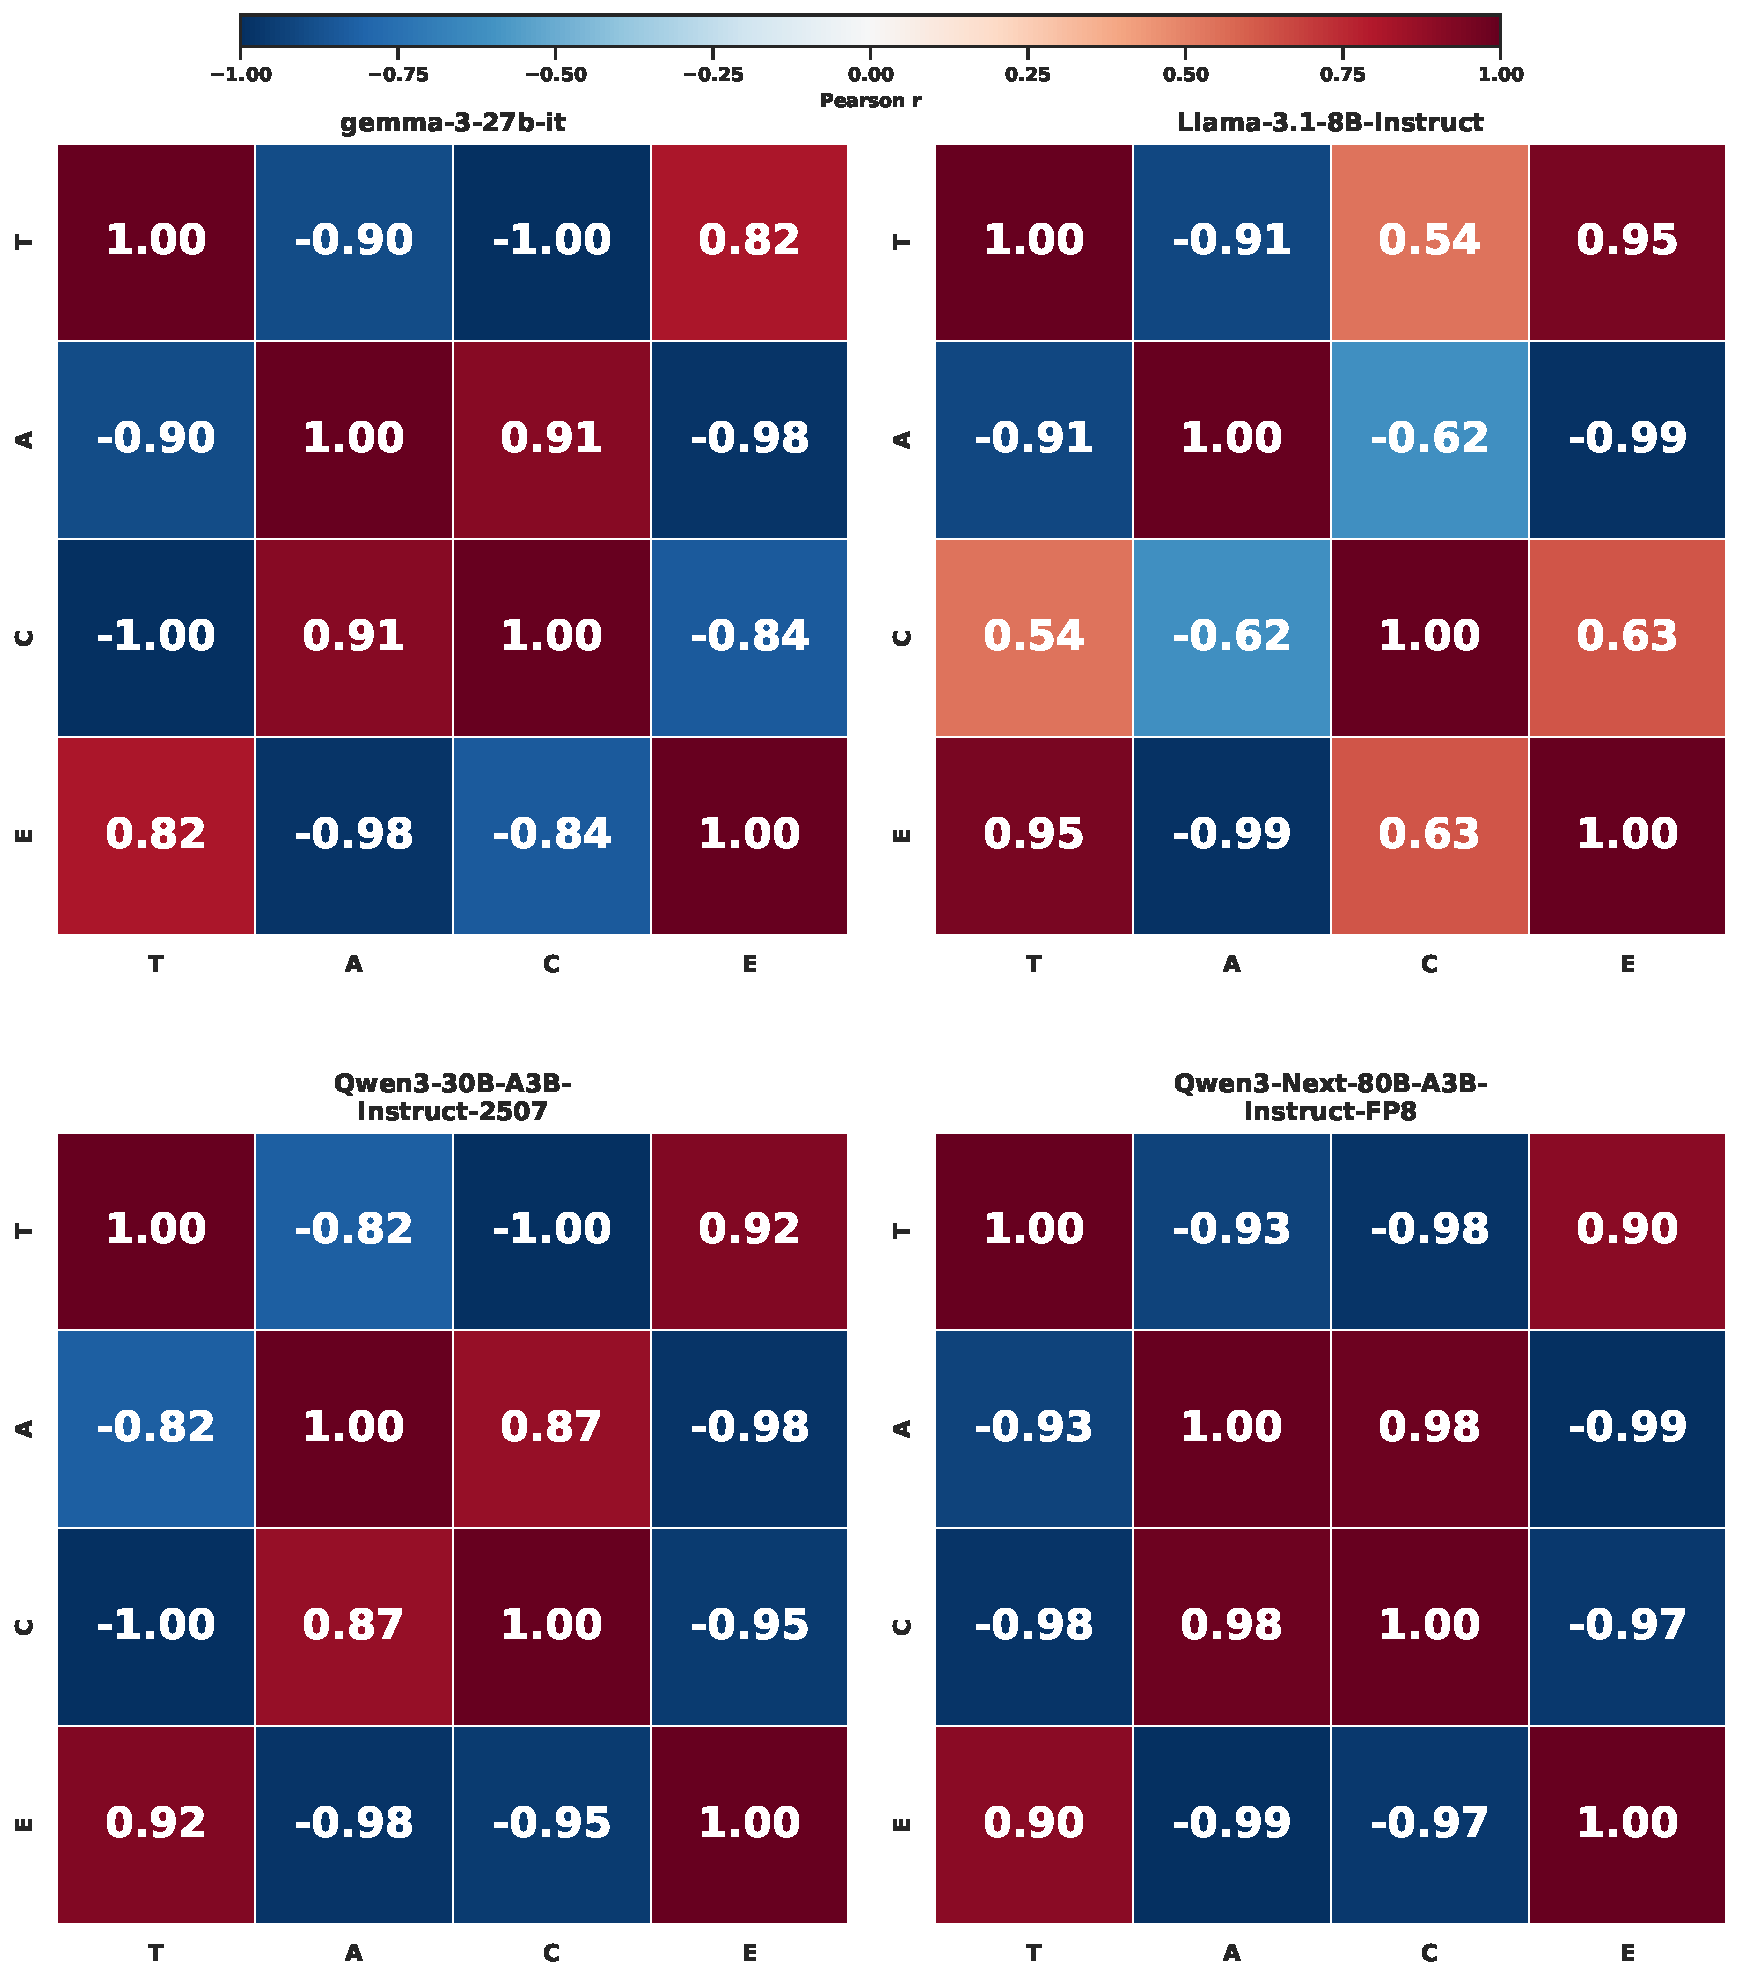
\includegraphics[width=1.0\linewidth]{photos/temperature_metric_correlation_heatmaps_TACE.pdf} 
    \caption{Pearson correlation matrices between decoding temperature (T) and evaluation metrics—agreement (A), consistency (C), and error rate (E)—across four LLMs.}
    \label{fig:correlation_analysis}
\end{figure}

Finally, in the context of LLM-as-a-Judge, the degradation of 
\textit{Error Rate} and \textit{Consistency} at high temperatures is 
itself a valuable diagnostic signal, as it exposes the fragility 
boundaries of the model Judge.  At low temperatures, the standard deviation is minimal; at high 
temperatures, it increases sharply, indicating that Judge outcomes 
for the same input become highly unstable.
The standard deviation of \texttt{gemma-3-27b-it} remains relatively 
small at high temperatures, whereas that of \texttt{Qwen3-Next-80B} 
is substantially larger. This reveals a structural difference in the two models' sensitivity 
to temperature perturbation---a finding that warrants further 
investigation. It also implies that \textbf{model selection} should be informed by 
model-specific characteristics, as well as by whether output 
diversity is desired.


As shown in Figure~\ref{fig:correlation_analysis}, increasing temperature \(T\) leads to a consistent decrease in Agreement \(A\) (strong negative correlation, \(-0.82\) to \(-0.93\)) and a marked increase in Error \(E\) (strong positive correlation, \(0.82\) to \(0.95\)), indicating reduced evaluation reliability at higher temperatures.  For \textit{Gemma-27b}, \textit{Qwen3-30B}, and \textit{Qwen3-Next-80B}, we observe near-perfect negative correlations between \(T\) and Consistency \(C\) (\(-0.98\) to \(-1.00\)), as well as between \(A\) and \(E\) (\(-0.98\) to \(-0.99\)), suggesting highly stable and consistent behavior across models. In contrast, \textit{Llama-3.1-8B-Instruct} deviates from this pattern, showing a positive correlation between \(T\) and \(C\) (\(r = 0.54\)) and between \(C\) and \(E\) (\(r = 0.63\)). This behavior suggests that, as a smaller model, its judgments are closer to random guessing, making them more sensitive to variations in random seeds.

















% \subsection{Temperature On Bias}

% Human Alignment bias

% Position Bias

% Verbosity Bias


% \subsection{Exploring Reasoning Models}



\subsection{Case Study}
\paragraph{Temperature on Judge Personas} We compare multiple high-temperature and low-temperature responses to the same judge cases. Our analysis clearly reveals that at high temperatures, LLMs exhibit a tendency toward more comprehensive analysis, which hinders their effectiveness as judges. This overthinking often leads to indecisiveness in final decisions, resulting in substantial variability in 10 repeated tests. In contrast, at low temperatures (including $T=0$) or even with CoT prompting, LLMs typically arrive at conclusions directly, fixate on a single salient point for stark comparisons, and reach decisions rapidly. Consequently, we hypothesize that the decline in judging performance at high temperatures---beyond parsing errors (primarily due to incomplete adherence to JSON output instructions)---largely stems from more thorough analysis, fostering greater indecisiveness. Low-temperature LLMs resemble irresponsible judges eager to expedite task completion, whereas high-temperature LLMs act as indecisive yet thorough evaluators. For more details on the response, see Appendix~\ref{sec:high vs low}.

\paragraph{Confusion at Low Temperatures}  A case-by-case inspection reveals that at higher temperatures, the model’s ability to adhere to the required JSON format degrades substantially, consistent with the observed increase in error rates: the model may omit the judge’s reasoning or fail to produce valid JSON outputs. Unexpectedly, even at low temperatures (\(T = 0.01\) and \(1.0\)), we still observe a non-negligible rate of formatting violations. This suggests that output randomness in LLMs is not fully eliminated under low-temperature decoding. These findings indicate that, in LLM-as-a-Judge settings, varying random seeds and temperature values can be useful for exposing variability and obtaining more robust evaluation signals.


\paragraph{Naturalistic Expression} We observe that higher temperatures lead to more diverse and less constrained generation patterns, which resemble more naturalistic and spontaneous expression, as shown in the following LLM response. In this regime, model outputs exhibit increased variability and fragmentation—phenomena that are largely absent under low-temperature settings. By contrast, low-temperature decoding results in more deterministic and instruction-following behavior. As temperature increases, the model becomes less strictly constrained by the prompt and exhibits greater exploratory behavior in its outputs. For qualitative examples, see Appendix~\ref{sec:llm_response_different_temp}.

\begin{responsebox}{LLM Response}
Assistant A correctly assigned ratings based on each review's sentiment. 
Review 1 ("phenomenal", 5-point scale) → 5; 
Review 2 ("unfortunately poor and predictable", described as "worst") → 1; 
Revision of "okay", "forgettable" → 2, which corresponds to a midrange score (around 1.5–2.5 out of 5),
similar to the "middle ground" rating 3. 

Assistant B incorrectly assigned the scores. 
\textbf{Review A, clearly very positive, deserves a 5, while "worst... in 2022" is a negative review (hence 1).} 
However, Assistant B gave review 2 a score of 3 (average or neutral?), even though it was clearly negative. 
Review 3 described the work as mediocre—thus a middle-ground rating around 2 or 3 would be appropriate. 
Instead, Assistant B assigned it a 1, the opposite of what was written.
\end{responsebox}


\subsection{Ensemble Thermo-judge}

We observe that LLMs can exhibit distinct \textit{judge personas} under varying temperature settings. To exploit this phenomenon, we propose a straightforward approach, termed \textbf{Ensemble Thermo-Judge}. Given an input query $x$, the judge model is executed $N$ times across one or multiple temperature configurations, yielding a collection of verdicts. A majority voting scheme is then applied, with the predominant verdict selected as the final decision. Compared to single-pass evaluation, this method leverages temperature-induced variability to enhance robustness and improve decision stability.

We partition the dataset into \textbf{Ambiguous} and \textbf{Non-ambiguous} subsets. A sample is designated as \textbf{Ambiguous} if and only if it satisfies both of the following criteria:
(1) \textit{low-temperature consistency}: under $T = 0.01$, 10 repeated evaluations yield verdicts (A/B/C) with Shannon entropy (in bits) below $0.01$;
(2) \textit{high-temperature disagreement}: the average Shannon entropy over $T \in \{1.5, 2.0, 3.0\}$ is greater than $0.50$ bits.
Samples that meet both criteria are assigned to the Ambiguous subset (42.6\%), whereas all remaining samples are categorized as Non-ambiguous.

We evaluate using a set of configurations that vary temperature \(T\) and sample size \(N\): \textbf{SP-Low} (\(T{=}0.01, N{=}1\)), \textbf{SP-Mid} (\(T{=}1.0, N{=}1\)), \textbf{Ens-Low} (\(T{=}0.01, N{=}10\)), \textbf{Ens-High} (\(T \in \{1.5, 2.0, 3.0\}, N{=}10\) per temperature), and \textbf{Ens-Mixed} (all \(T \neq 0.01\), with 3 runs per temperature, \(N{=}15\) total). Here, \textbf{SP} (single-pass) denotes a single stochastic generation (\(N=1\)) at a given temperature, while \textbf{Ens} (ensemble) denotes aggregating multiple independent generations (\(N>1\)) via majority voting. Ensemble Thermo-Judge combines temperature-induced diversity with majority voting to yield more robust and reliable judgments, particularly for ambiguous cases.




\begin{table}[t]
\centering
\small
\begin{adjustbox}{width=\columnwidth,center}
\begin{tabular}{l c c c c}
\toprule
Subset & \(T\) & \textit{Mean Entropy} & \textit{Flip Rate} & \textit{Lift} \\
\toprule
\rowcolor{gray!5}
\multirow{6}{*}{\textbf{Ambiguous}}
& 0.01 & 0.0000 & 0.0000 & 0.0000 \\
& 0.50 & 0.1722 & 0.0323 & 0.1722 \\
& 1.00 & 0.3298 & 0.0484 & 0.3298 \\
& 1.50 & 0.5720 & 0.0710 & 0.5720 \\
& 2.00 & 0.8068 & 0.1161 & 0.8068 \\
& 3.00 & \textbf{1.1003} & \textbf{0.2968} & \textbf{1.1003} \\
\midrule
\rowcolor{gray!8}
\multirow{6}{*}{\textbf{Non-Ambiguous}}
& 0.01 & 0.0517 & 0.0000 & 0.0000 \\
& 0.50 & 0.0540 & 0.0190 & 0.0022 \\
& 1.00 & 0.0630 & 0.0214 & 0.0112 \\
& 1.50 & 0.0681 & 0.0196 & 0.0165 \\
& 2.00 & 0.0979 & 0.0268 & 0.0462 \\
& 3.00 & \textbf{0.2709} & \textbf{0.0410} & \textbf{0.2192} \\
\bottomrule
\end{tabular}
\end{adjustbox}
\caption{Performance across temperatures for Ambiguous and Non-Ambiguous subsets. \textit{Mean Entropy}: average Shannon entropy of verdicts; \textit{Flip Rate}: fraction of majority changes w.r.t. \(T{=}0.01\); \textit{Lift}: entropy increase over \(T{=}0.01\). Bold indicates the maximum within each subset and metric.}
\label{tab:exp1f_single_max_per_group}
\end{table}

\subsubsection{Ambiguity Indicator}

As shown in Table~\ref{tab:exp1f_single_max_per_group}, Ambiguous samples exhibit a pronounced sensitivity to temperature. Specifically, verdict entropy increases substantially as temperature rises, reaching approximately 0.8--1.0 bits at higher temperatures. Concurrently, the flip rate escalates sharply to 40--50\%, and disagreement lift grows monotonically with temperature. In contrast, Non-ambiguous samples remain comparatively stable across all evaluated metrics. Their entropy shows only a marginal increase, flip rates remain below 10--15\%, and consistency deteriorates minimally, indicating that their judgments are largely insensitive to temperature variations. Overall, a low temperature setting (\(T = 0.01\)) induces a form of ``spurious certainty,'' wherein the model produces highly consistent yet not necessarily reliable judgments due to constrained output variability. Conversely, higher temperatures more effectively reveal the underlying uncertainty in Ambiguous cases, while exerting minimal adverse effects on inherently clear (Non-ambiguous) samples.


\subsubsection{Turning Up the Heat}

These observations motivate the design of temperature-aware judgment strategies, which we further instantiate and evaluate under the proposed Ensemble Thermo-Judge framework. Notably, high-temperature settings may adversely affect the model’s instruction-following capability; for example, they can destabilize adherence to the required JSON output format, a common constraint in LLM-based evaluation pipelines. To isolate the negative effect of temperature on LLM instruction following behaviors, we explicitly analyze this class of format-related errors and exclude any samples that violate the prescribed output format from the Thermo-Judge voting set within the ensemble. This filtering procedure enables a cleaner assessment of the impact of high-temperature settings on judgment outcomes, free from confounding factors introduced by format inconsistencies or related artifacts.

\begin{table}[htbp]
\centering
\small
\begin{adjustbox}{width=\linewidth}
\begin{tabular}{lcc}
\toprule
Pipeline & AGR (Amb) & AGR (Non-Amb) \\
\midrule
\rowcolor{gray!5}
\multicolumn{3}{l}{\textbf{Direct}} \\
\addlinespace[2pt]
SP-Low (T=0.01, N=1)    & 0.5141 & 0.6568 \\
SP-Mid (T=1.0, N=1)     & 0.5094 & 0.6551 \\
Ens-Low (T=0.01, N=10)  & 0.5188 & 0.6568 \\
Ens-High (T=1.5, N=10)  & 0.5235 & 0.6551 \\
Ens-High (T=2.0, N=10)  & \textbf{0.5305} & 0.6568 \\
Ens-High (T=3.0, N=10)  & 0.5258 & 0.6551 \\
Ens-Mixed (Mix-T, N=15) & 0.5070 & \textbf{0.6585} \\

\midrule
\rowcolor{gray!5}
\addlinespace[1pt]
\multicolumn{3}{l}{\textbf{Chain-of-Thought}} \\
\addlinespace[2pt]
SP-Low (T=0.01, N=1)    & 0.4413 & 0.6456 \\
SP-Mid (T=1.0, N=1)     & 0.4240 & 0.6578 \\
Ens-Low (T=0.01, N=10)  & 0.4413 & 0.6456 \\
Ens-High (T=1.5, N=10)  & 0.4507 & \textbf{0.6649} \\
Ens-High (T=2.0, N=10)  & 0.4484 & 0.6551 \\
Ens-High (T=3.0, N=10)  & \textbf{0.4682} & 0.6394 \\
Ens-Mixed (Mix-T, N=15) & 0.4076 & 0.6573 \\

\bottomrule
\end{tabular}
\end{adjustbox}
\caption{
Performance comparison between standard direct prompting and CoT. Results are reported on ambiguous (Amb) and non-ambiguous (Non-Amb) subsets. Bold indicates the best result within each group.
}
\label{tab:exp2_baseline_cot_block}
\end{table}

As shown in Table~\ref{tab:exp2_baseline_cot_block}, the impact of temperature is more pronounced on the Ambiguous subset under the Baseline configuration, particularly when high-temperature sampling is combined with ensemble decoding. Under single-pass inference, SP-Low (\(T=0.01, N=1\)) achieves an AGR of 0.51, while SP-Mid (\(T=1.0, N=1\)) yields a comparable AGR of 0.50, suggesting that varying temperature alone does not consistently improve performance in a single-pass setting. In contrast, when elevated temperatures are coupled with repeated sampling, performance improves consistently: Ens-High (\(T=1.5, N=10\)) reaches 0.52, \(T=2.0\) further improves to 0.53, and \(T=3.0\) remains competitive at 0.52. Although the absolute gains are modest, the consistent improvement indicates that the additional diversity introduced by higher temperatures can be effectively exploited via majority voting. This suggests that such gains are particularly relevant for long-tail or ambiguous cases, where comprehensive exploration of the decision space is beneficial for more reliable judgments.

In addition, CoT shows weaker overall performance on the Ambiguous subset, but high-temperature ensemble decoding yields the most substantial gains within the CoT setting. While single-pass inference offers little benefit—SP-Low (\(T=0.01, N=1\)) reaches 0.44 and SP-Mid (\(T=1.0, N=1\)) drops to 0.42—introducing high-temperature sampling with ensembling leads to clear improvements. Ens-High (\(T=1.5, N=10\)) increases AGR to 0.45, \(T=2.0\) reaches 0.45, and \(T=3.0\) achieves 0.47, representing the strongest performance for CoT. Although these gains remain below the Baseline peak of 0.53, the relative improvement from high-temperature ensembling is noticeably larger for CoT than for single-pass methods, indicating that CoT particularly benefits from the exploratory signal introduced by higher temperatures in challenging, ambiguous cases. Interestingly, this finding challenges the common assumption that higher temperatures are inherently detrimental. In the LLM-as-a-Judge setting, elevated temperatures can instead yield consistent gains when combined with ensembling. We hypothesize that this effect may stem from the increased diversity induced by high-temperature sampling, which allows the model to explore a broader range of implicit reasoning paths or “personas,” potentially leading to more comprehensive and robust judgments.


\section{Conclusion}

This work conducts large-scale controlled experiments to systematically investigate the impact of temperature on the performance of LLMs as evaluators, providing actionable guidance for both industrial practice and future research on temperature effects. \textbf{Our findings demonstrate that low-temperature settings yield near-perfect consistency and negligible error rates, whereas higher temperatures lead to substantial degradation in consistency and a sharp increase in error rates.} These effects vary across model types, evaluation paradigms, and prompting strategies. Quantitatively, temperature exhibits a strong negative correlation with consistency and a strong positive correlation with error rates, indicating that it is a primary determinant of evaluation reliability rather than a negligible engineering detail.

Beyond these general trends, aggregate statistics and case studies reveal nuanced benefits of higher temperatures. \textbf{Specifically, elevated temperatures can expand both the depth and breadth of reasoning exhibited by LLM evaluators and alter their judgment patterns.} Contrary to the common assumption that high-temperature outputs merely reflect unstructured or illogical hallucinations, our analysis shows that such models do engage in structured reasoning, but frequently deviate from task instructions, thereby increasing parsing errors and reducing overall performance. Notably, instruction violations are not entirely eliminated even under low-temperature settings, challenging the prevailing view that low temperature is universally optimal for evaluation tasks. Consequently, higher temperatures become meaningful in scenarios requiring deeper or more exploratory reasoning, although they should be paired with multiple sampling runs under different random seeds.

Furthermore, by partitioning the evaluation set into Ambiguous and Non-Ambiguous subsets—where the former comprises inherently more challenging cases—we observe that temperature exerts a substantially greater influence on the Ambiguous subset, while having minimal impact on the Non-Ambiguous subset. This observation suggests that performance variations across temperature settings can serve as an implicit indicator of instance-level ambiguity. \textbf{Building on this insight, we evaluate a simple yet effective method, Ensemble Thermo-Judge, on the Ambiguous subset, demonstrating that repeated high-temperature judgments improve AGR.} Additionally, we find that CoT achieves better performance at higher temperatures within this subset, further supporting the utility of diversified temperature configurations. In practical terms, when stability, reproducibility, and cost efficiency are the primary concerns, low-temperature settings are strongly recommended. In contrast, for complex evaluation scenarios that require nuanced, multi-perspective reasoning or deeper deliberation, higher temperatures offer tangible advantages.

\section{Limitations}

We outline several limitations of this study. First, we restrict our experiments to open-source models. This choice is primarily driven by the need for transparent and controllable temperature configurations, which are not consistently available in closed-source systems. While this may limit direct coverage of proprietary models, the controlled setting allows us to isolate and systematically analyze temperature effects, and we expect the qualitative trends to generalize across model families.

Second, inference outcomes may vary with random seeds, temperature settings, and hardware environments. This effect becomes more pronounced at higher temperatures (up to \(T = 3.0\) in our experiments), where generation is inherently more stochastic. Even with identical seeds and decoding parameters, minor differences in floating-point computations across GPU architectures can occasionally lead to divergent outputs. Importantly, our results are based on aggregate statistics over multiple runs, which mitigates the impact of such variability. Exploring even higher temperature regimes remains an interesting direction for future work.

Third, our evaluation relies on two datasets with different characteristics. For MMLU\_Pro, the ``golden'' labels are produced by a strong closed-source model rather than human annotation. While this introduces potential biases, such labels are widely adopted in prior work and provide a consistent and scalable evaluation signal. Taken together, these datasets provide a balanced perspective, though further validation on fully human-annotated benchmarks would strengthen future studies.

For future work, a promising direction for improving judgment quality—particularly in agent-based systems—is to combine a high-temperature agent for exploratory initial judgments with a low-temperature agent for output refinement, thereby balancing reasoning diversity with determinism. More broadly, these findings advocate for task-adaptive temperature strategies in LLM evaluation pipelines, moving beyond fixed low-temperature defaults to enhance robustness. We do not explore the interaction between temperature and various evaluator biases, which remains an open research question.

\bibliography{custom}




\appendix

\section{Supplementary Causal Analysis}

\subsection{Causal Effect Estimation}

Intuitive statistical analyses cannot fully capture the direct causal influence of temperature on the judge. 
They can only empirically identify correlations without determining whether such relationships are driven by other factors, such as the prompt. 
To address this limitation, we formulate the analysis within the potential outcomes framework. 
For each item \( i \), let \( Y_i(t, X) \) denote the potential outcome under temperature \( t \), 
where \( X \) represents all confounders and moderators. 
Our primary estimand is the conditional causal effect of temperature:
\[
  \tau(t, t' \mid p, l)
  = \mathbb{E}\!\left[Y_i(t, X) - Y_i(t', X)\right].
\]

In this framework, the co-variates \( X \) include \textit{Judge Type}, \textit{Prompt Variant}, and \textit{Model}, 
while the treatment variable corresponds to the temperature parameter. 
We define the binary treatment indicator as
\[
  T_i = 1\!\left[t_i \ge 1.5\right],
\]
where \( T_i = 1 \) indicates a high-temperature sample (\( t_i \ge 1.5 \)), 
and \( T_i = 0 \) corresponds to a low-temperature sample (\( t_i < 1.5 \)).

For causal estimation, we employ a 3-Fold Cross-Fitted Augmented Inverse Probability Weighting 
(Cross-Fitted AIPW; see \cite{chernozhukov2024doubledebiasedmachinelearningtreatment}) estimator 
to estimate the Average Treatment Effect (ATE). 
Within each training fold, three Light Gradient Boosting Machine (LightGBM) regressors are fitted 
to predict propensity scores and potential outcomes. In addition, a Shapley value attribution analysis is conducted to examine the magnitude of the effects of temperature and other moderators on model performance.


\subsection{Causal Effect Analysis}


\begin{figure*}[h]
    \centering
    \hspace{-1cm}  
    \adjustbox{max width=1.0\textwidth, max totalheight=0.70\textheight, center}{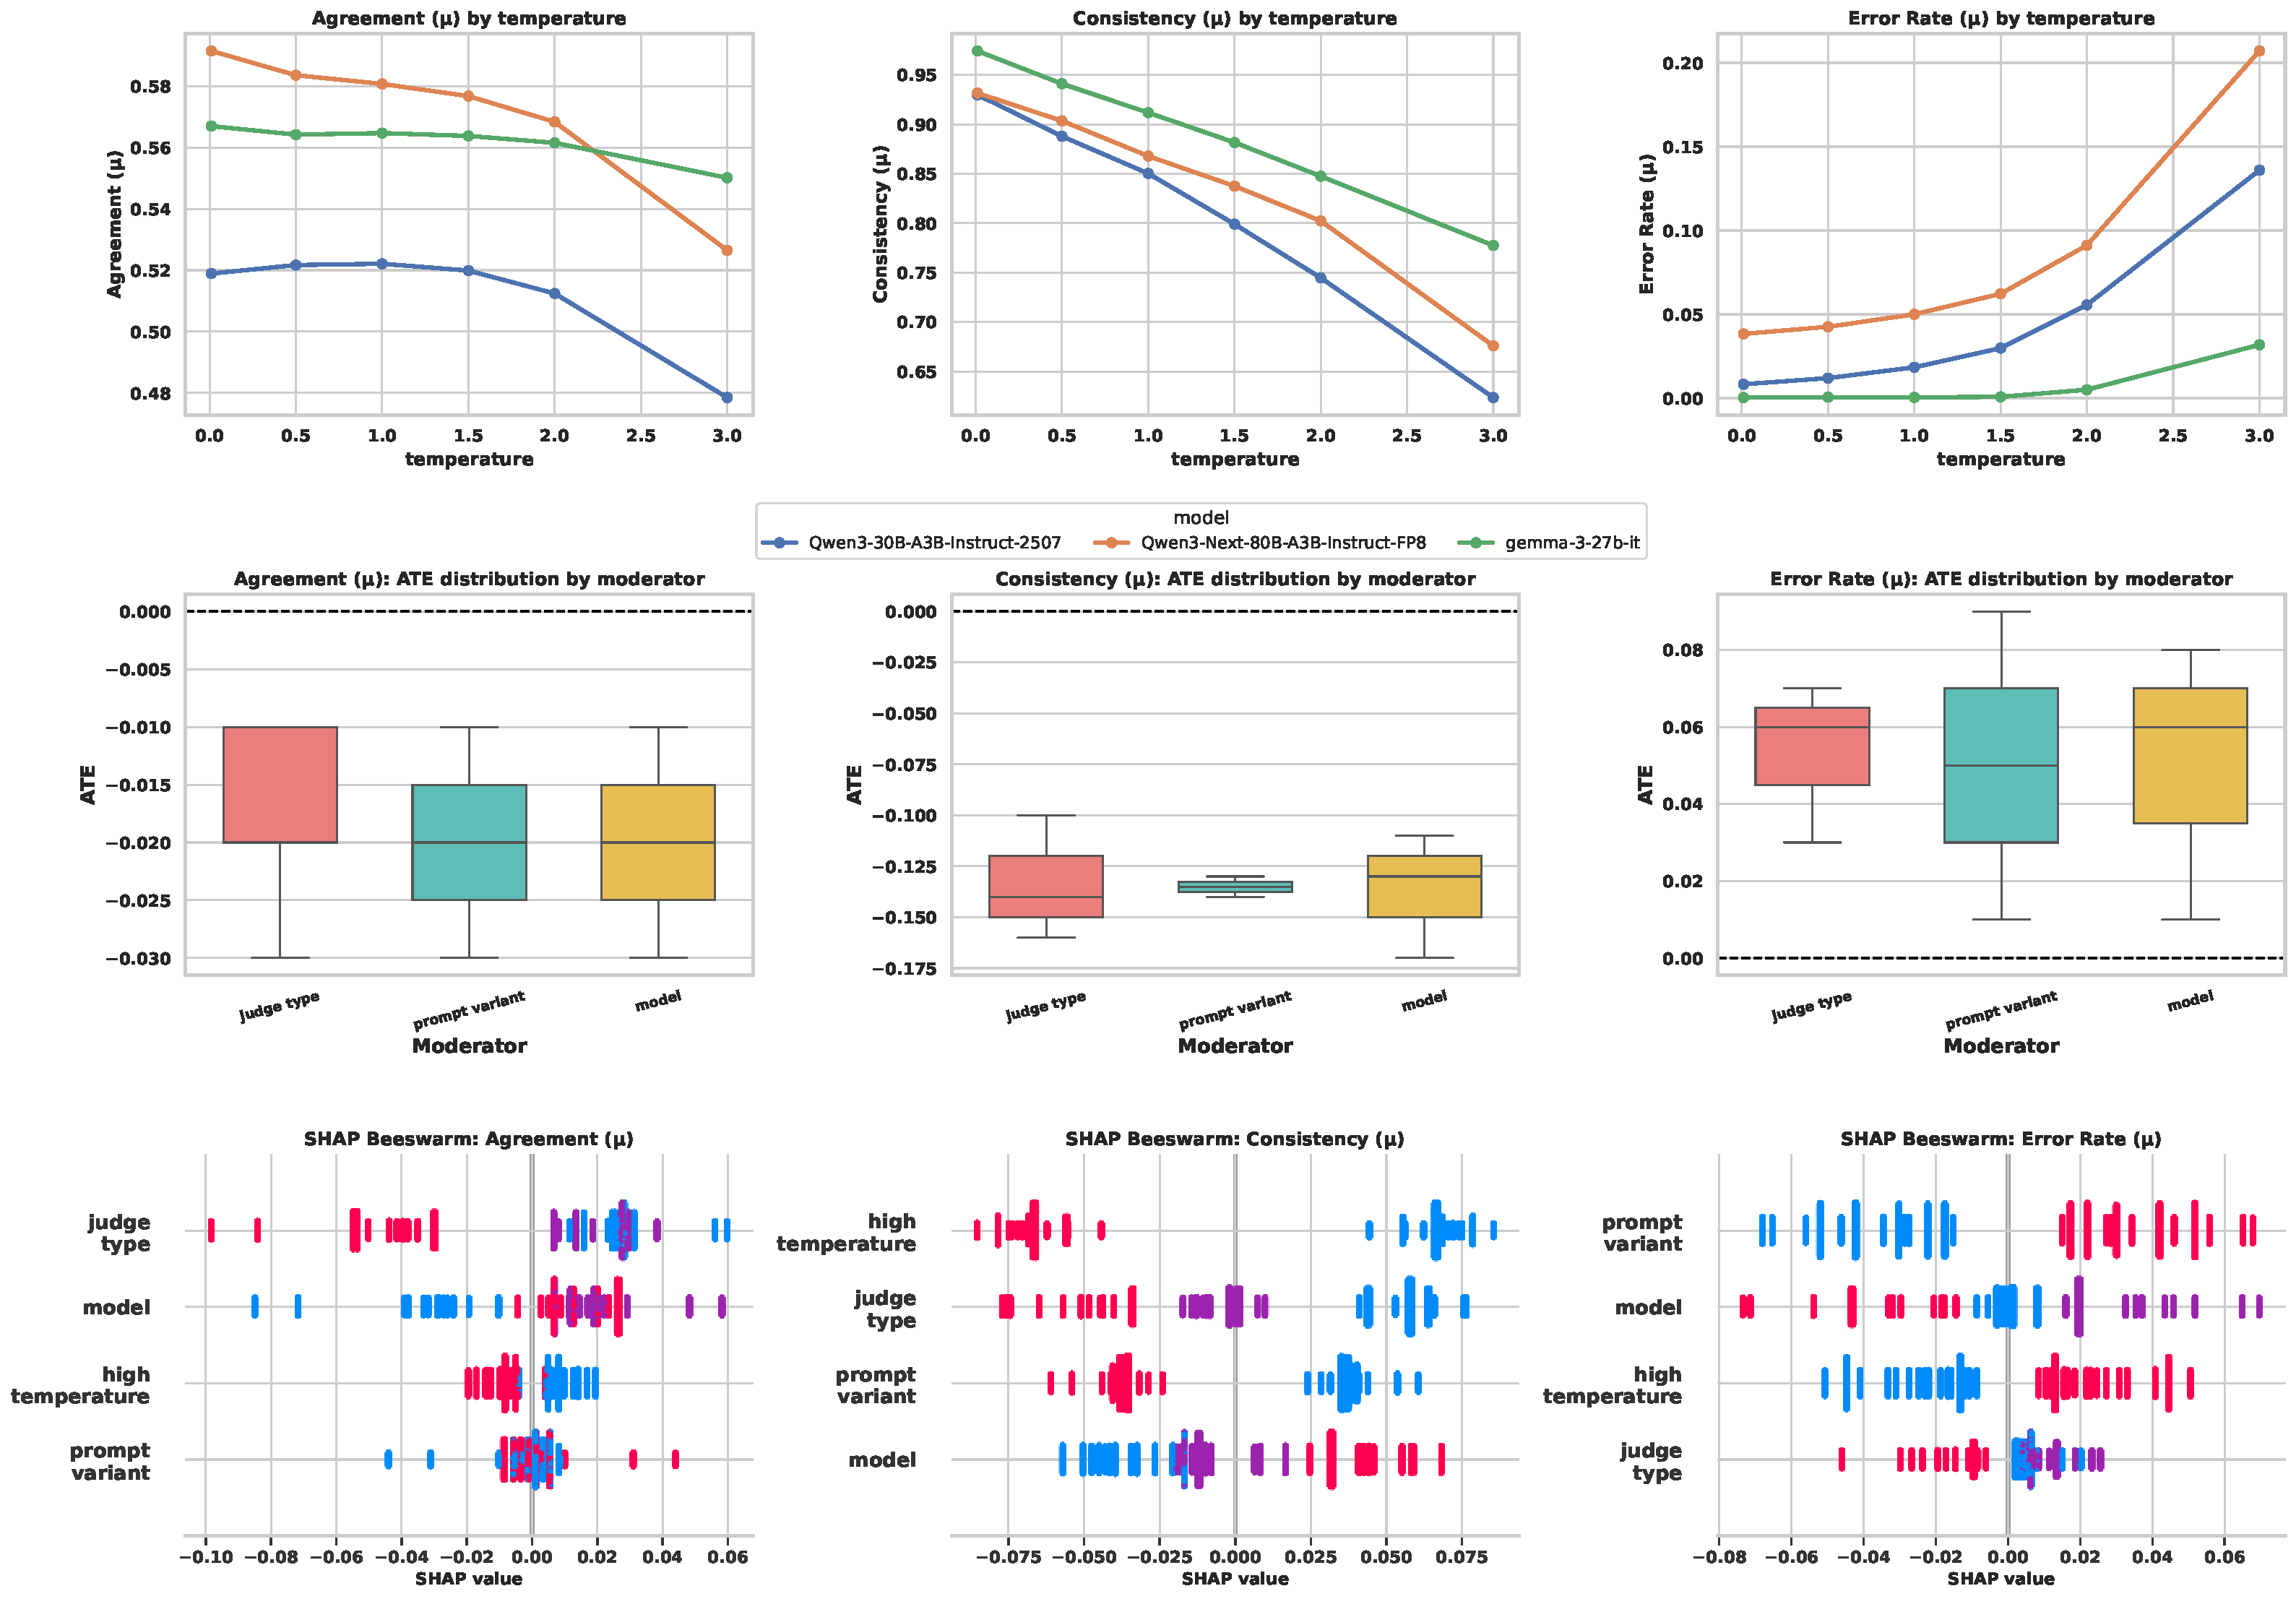
\includegraphics{photos/ate_boxplot_temperature_trends_shap_3x3.pdf}}
    \caption{\textbf{Comprehensive ATE Analysis Across Moderators, Temperature, and Feature Importance.}
    \textbf{Row 1:} Temperature trends of different models (shared legend), showing mean tendencies across temperature ranges (lines indicate averages, not ATE values).
    \textbf{Row 2:} Boxplots of Average Treatment Effect (ATE) distributions across three moderators for each outcome metric (dashed line denotes ATE = 0).
    \textbf{Row 3:} SHAP beeswarm plots ranking feature importance by impact magnitude for each outcome metric.
    All panels share consistent bold styling and bright color palettes for clarity.}
    \label{fig:causal analysis}
\end{figure*}

The increase in temperature is indeed statistically negatively correlated with performance. However, different prompt settings, judge type configurations, and model choices also influence how temperature affects these three metrics. Therefore, a causal analytical approach is required to draw valid conclusions.


As shown in Figure~\ref{fig:causal analysis}, the first row illustrates the association between temperature and the three metrics. For the three models, \textit{Agreement} decreases slightly as temperature increases, \textit{Consistency} exhibits a more pronounced decline, and \textit{Error Rate} rises substantially after an initially stable phase. Therefore, higher temperatures substantially harm Consistency and increase Error Rate, while their effect on Agreement is directionally stable but relatively small in magnitude. Notably, for Qwen3-30B-A3B-Instruct-2507, increasing temperature actually improves the judge's Agreement performance, whereas the significant rise in Error Rate tends to degrade Agreement. 
This suggests that the increase in Error Rate induced by higher temperature is an important factor behind the overall decline in Agreement. 
Thus, how to mitigate the errors generated under higher temperatures may become an interesting research direction for LLMs as judges.


The second row of Figure~\ref{fig:causal analysis} shows under which conditions the temperature causal effect is stronger or weaker (more causal effect analysis, see Appendix~\ref{sec:appendix_ate}). For Agreement, the group-level ATEs are mostly in the range $-0.03$ to $-0.01$, with small dispersion; 
for Consistency, the group-level ATEs range from $-0.17$ to $-0.10$, indicating more pronounced heterogeneity; 
for Error Rate, the group-level ATEs lie between $+0.01$ and $+0.09$, with the largest variation across \texttt{prompt\_variant}, where higher temperature consistently leads to an increase in error rate. 
In particular, the strength of the temperature effect varies the most across different prompting strategies, while other factors remain relatively fixed. 
Therefore, when the temperature is set higher, the system tends to be more inconsistent and more prone to errors overall. 
CoT requires more extensive text generation and thus tends to amplify the negative impact of temperature on judge performance.



The SHAP beeswarm plots (third row) illustrate both the magnitude and direction of each feature’s contribution to the outcome models. For \textit{Agreement}, the predictions are primarily influenced by \texttt{judge type} ($+0.0324$) and \texttt{model} ($+0.0251$), whereas \texttt{temperature} plays a minor role ($+0.0089$). For \textit{Consistency}, \texttt{temperature} emerges as the most influential factor ($-0.0665$), clearly dominating all other features. For \textit{Error Rate}, \texttt{prompt\_variant} exerts the strongest effect ($+0.0371$), followed by \texttt{temperature} ($+0.0249$). Moreover, the bootstrap standard errors are consistently small (mostly within the range of 0.0004 to 0.002), indicating high estimation stability. These results suggest that \texttt{temperature} ranks among the top two factors influencing judge performance. When \textit{Agreement} is prioritized, \texttt{judge type} and \texttt{model} are the primary determinants; however, when \textit{Consistency} is of greater concern, \texttt{temperature} warrants substantially more attention.




\section{Prompt For Generating Gold Judge Labels}
\label{appendix:judge_prompt_4.5}

To evaluate the MMLU-Pro dataset in the absence of human judges results, we employ the state-of-the-art (SOTA) GPT-5.4 model as an automated judge. 
The evaluation protocol, illustrated in the following prompt box, determines the superior response between two model outputs or declares a tie when performance is deemed equivalent.




\begin{promptbox}{System Prompt Template}
You are an impartial judge evaluating answers to multiple-choice questions.  
Your task is to decide which answer is better or whether they are equally good.

Respond \textbf{ONLY} with a JSON object — no markdown, no extra text — in this exact format:

\{"winner": "<A|B|tie>", "reason": "<one concise sentence>"\}
\end{promptbox}


\begin{userbox}{User Prompt Template}
\textbf{Question:}
\texttt{[question text]}

\textbf{Options:}
\texttt{A. [option A]}
\texttt{B. [option B]}
\texttt{...}

\textbf{Correct Answer:}
\texttt{[correct answer]}

\textbf{Answer A (model: [modelA]):}
\texttt{[answer A content]}

\textbf{Answer B (model: [modelB]):}
\texttt{[answer B content]}

Which answer is better? Reply with JSON only.
\end{userbox}


\section{Prompt Template For Judge}
\label{appendix:prompt template}

\begin{userbox}{Pairwise Comparison Direct Judge Prompt}
You are a fair and impartial judge. Your task is to evaluate two AI assistant responses to a user question and decide which one is better.

Respond ONLY with valid JSON using exactly one key:
\begin{verbatim}
{"judge result":"A"}
\end{verbatim}

Use ``A'' if assistant A is better, ``B'' if assistant B is better, and ``C'' for a tie.
Do not output any additional keys, explanation, markdown, or text.
\end{userbox}

\begin{userbox}{Pairwise Comparison COT Judge Prompt}
You are a fair and impartial judge. Your task is to evaluate two AI assistant responses to a user question. First, compare them on helpfulness, relevance, accuracy, depth, and creativity. Then compare them on coherence, clarity, and language quality. Finally, give your verdict.

Respond ONLY with valid JSON using exactly these two keys:
\begin{verbatim}
{"judge reason":"<brief explanation>"
,"judge result":"A"}
\end{verbatim}

Use ``A'' if assistant A is better, ``B'' if assistant B is better, and ``C'' for a tie.
Do not output markdown or any extra text outside the JSON object.
\end{userbox}

\begin{userbox}{Reference Guided Grading Direct Judge Prompt}
Please act as an impartial judge and evaluate the quality of the responses provided by two AI assistants to the user question displayed below. Your evaluation should consider correctness and helpfulness. You will be given a reference answer, assistant A's answer, and assistant B's answer. Your job is to evaluate which assistant's answer is better. Begin by comparing both assistants' answers with the reference answer. Identify mistakes if needed. Avoid position bias, length bias, and any bias toward assistant names.

Respond ONLY with valid JSON using exactly one key:
\begin{verbatim}
{"judge result":"A"}
\end{verbatim}

Use ``A'' if assistant A is better, ``B'' if assistant B is better, and ``C'' for a tie.
Do not output any additional keys, explanation, markdown, or text.
\end{userbox}

\begin{userbox}{Reference Guided Grading COT Judge Prompt}
Please act as an impartial judge and evaluate the quality of the responses provided by two AI assistants to the user question displayed below. Your evaluation should consider correctness and helpfulness. You will be given a reference answer, assistant A's answer, and assistant B's answer. Your job is to evaluate which assistant's answer is better.

First, compare assistant A's answer and assistant B's answer against the reference answer for correctness, completeness, and helpfulness. Then identify any mistakes, omissions, or misleading claims in each answer. Finally, compare the two assistants directly and explain which answer is better overall, while avoiding position bias, length bias, and any bias toward model names.

Respond ONLY with valid JSON using exactly these two keys:
\begin{verbatim}
{"judge_reason":"<brief explanation>"
,"judge result":"A"}
\end{verbatim}

Use ``A'' if assistant A is better, ``B'' if assistant B is better, and ``C'' for a tie.
Do not output markdown or any extra text outside the JSON object.
\end{userbox}

\begin{userbox}{Single Answer Grading Direct Judge Prompt}
You are a fair and impartial judge. Rate the quality of the AI assistant's response to the user question on a scale of 1 to 10.

Respond ONLY with valid JSON using exactly one key:
\begin{verbatim}
{"judge result":7}
\end{verbatim}

The value of \texttt{judge\_result} must be an integer between 1 and 10.
Do not output any additional keys, explanation, markdown, or text.
\end{userbox}

\begin{userbox}{Single Answer Grading COT Judge Prompt}
You are a fair and impartial judge. Rate the quality of the AI assistant's response to the user question on a scale of 1 to 10. First analyze the response's helpfulness, relevance, accuracy, depth, creativity, and coherence. Then provide your rating.

Respond ONLY with valid JSON using exactly these two keys:
\begin{verbatim}
{"judge_reason":"<brief explanation>"
,"judge result":7}
\end{verbatim}

The value of \texttt{judge\_result} must be an integer between 1 and 10.
Do not output markdown or any extra text outside the JSON object.
\end{userbox}


\section{Examples}
\subsection{High Temperature Vs Low Temperature}
\label{sec:high vs low}

This response from Qwen3-30B-A3B-Instruct-2507 is more direct and more polite, yet considers fewer aspects and yields a more concise answer from the Judge.
\begin{responsebox}{LLM Response With T=0.01}

Assistant A's answer is incorrect. The probability is not 1/3. The correct approach is to calculate
the probability of the complementary event (rolling a total less than 3) and subtract it from 1. The
only outcome with a total less than 3 is (1,1), which gives a sum of 2. So the probability of
rolling a total of at least 3 is $1 - 1/36 = 35/36$. Assistant B correctly identifies all 36 possible
outcomes and correctly notes that only (1,1) results in a sum less than 3. However, Assistant B
makes a critical error by stating that all 36 outcomes result in a total of at least 3, which is
false. The outcome (1,1) gives a sum of 2, which is less than 3. Therefore, there are actually 35
favorable outcomes, not 36. The correct probability is $35/36$, not 1. Both assistants are incorrect,
but Assistant B provides a more thorough and correct reasoning process, even though the final
conclusion is wrong. Assistant A's answer is completely wrong in both reasoning and final answer.
Therefore, Assistant B is better despite the error in the final conclusion.
\end{responsebox}

This response, in contrast, provides more detailed information and a greater number of justifications for their judgment. When the temperature is set to a high value, the model does not produce nonsensical outputs or exhibit obvious hallucinations; instead, it offers a more detailed explanation of its analysis to make its decisions appear well grounded. Furthermore, the final conclusion reached is correct, which is highly significant because it reflects the meaningful role of the high‑temperature setting.

\begin{responsebox}{LLM Response With T=2.0}
Assistant A's answer contains a significant error: claiming the probability is 1/3 (33.3\%) is
incorrect. The only possible totals that are less than 3 are when rolling a 2. There is only one
outcome that produces a sum of 2: (1,1). Thus, the probability of rolling at least 3 is $35/36$, not
1/3. Additionally, Assistant A's justification (``probability of rolling a 3 or higher is 1/3 of the
total number of outcomes (6)'') is illogical and mathematically incorrect---total possible outcomes for
the sum are not 6, nor does the number 6 relate to the probability in the claimed manner.

Assistant B provides a comprehensive, accurate calculation using the sample space of all 36 possible
outcomes, correctly identifying that only (1,1) produces a sum less than 3, hence the probability of
rolling at least 3 is $35/36$. However, Assistant B incorrectly asserts that `there are 36 such
outcomes' and therefore the probability is $36/36=1$---an erroneous conclusion from overcounting. The
correct number of favorable outcomes (for sum $\geq$ 3) should be 35, not 36.

Although both answers contain calculation errors, Assistant B's reasoning process is vastly more
accurate in approach and method. It correctly lists and counts the full set of sample space
elements. The error in Assistant B's final tally (missing that (1,1) has sum of 2) seems to be a
lapse, but does not undermine the overall clarity and correctness of the reasoning path and
approach.

In comparison, Assistant A provides no such method, misidentifies the distribution completely, and
gives an obviously wrong probabilistic fraction.

Thus, B provides more helpful, relevant, and accurate reasoning and methodology---even if there is a
minor factual mistake in conclusion---making it vastly better overall than A.
\end{responsebox}

For the same question, this response is likewise reasonable with T=3.0. In my view, the Judge’s reasoning is more comprehensive, and its final decision of a tie suggests that it detected certain flaws in both responses, making it difficult to determine a clear winner. Consequently, it ultimately concludes with a tie.



\begin{responsebox}{LLM Response With $T=3.0$}
Assistant A's reasoning contains a critical error---claiming that rolling at least 3 has only a $1/3$ probability, with an incorrect basis that only considers a subset of totals ranging from 2 through 12. This ignores the combinatorially weighted outcomes for each value. The truth (as noted correctly by Assistant B) is that the only impossible case for a sum less than 3 is the sum~$2$, which corresponds to the single combination $(1,1)$ out of a total of 36 possible outcomes. Therefore, $(36 - 1)/36$ gives the final probability as $35/36$.

Furthermore, while Assistant B lists all 35/36 outcomes as acceptable, it initially includes the $(1,1)$ case, thus over‑counting by listing it. However, it clearly notes this incorrect listing and still arrives at the correct result that the probability equals nearly all but one of the 36 outcomes.

Thus both assistants present some flawed thinking. Assistant A, however, makes an incorrect assumption and provides far less precise and misleading data. The true and intended result is that the only impossible total is $2$, so the favorable outcomes correspond to all sums except $2$, giving a probability of $35/36$. Among the two, Assistant~B is preferable for its more structured methodology, thorough enumeration, and effective correction to the correct result.
\end{responsebox}


\subsection{LLM Response With Different Temperature}
\label{sec:llm_response_different_temp}

\subsubsection{Response Example 1}

\begin{responsebox}{LLM Response With $T=0.0$}
Assistant A correctly interprets the reviews and assigns appropriate scores: Review 1 is very
positive (5), but Assistant A gives it a 3, which is incorrect. Review 2 is very negative (1), and
Assistant A gives it a 1, which is correct. Review 3 is neutral/average (3), but Assistant A gives
it a 2, which is slightly low. However, Assistant B's response is completely reversed: Review 1 is
scored as 1 (very negative), which is wrong; Review 2 as 3 (neutral), which is incorrect; and Review
3 as 5 (very positive), which is also wrong. Therefore, Assistant A's answer, while not perfect, is
closer to correct than Assistant B's, which is entirely incorrect.
\end{responsebox}

\begin{responsebox}{LLM Response With $T=0.5$}
Assistant A correctly interprets the reviews and assigns appropriate scores: Review 1 is very
positive (5), but Assistant A assigns 3, which is incorrect. Review 2 is very negative (1),
correctly assigned. Review 3 is neutral (3), but Assistant A assigns 2, which is too low. Assistant
B incorrectly assigns 1 to the first review (which is very positive), 3 to the second (which is very
negative), and 5 to the third (which is neutral). Both assistants make errors, but Assistant A's
scores are closer to the correct interpretation. Review 1 is clearly very positive, so should be 5,
not 3. Review 3 is “okay” and “ordinary,” which is closer to neutral (3) than 2. Therefore,
Assistant A is better.
\end{responsebox}

\begin{responsebox}{LLM Response With $T=1.0$}
Assistant A correctly interprets the sentiment of each review and assigns appropriate scores: Review
1 is very positive (5), but Assistant A assigns 3, which is inaccurate. Review 2 is very negative
(1), and Assistant A assigns 1 correctly. Review 3 is neutral/average (3), but Assistant A assigns
2, which is slightly low. However, Assistant A's scores are closer to the intended sentiment.
Assistant B's response is completely incorrect: they reverse the sentiment values. Review 1 is
highly positive but assigned 1; Review 2 is negative but assigned 3; Review 3 is average but
assigned 5. This indicates a fundamental misunderstanding of the task. Therefore, Assistant A is
better despite minor inaccuracies.
\end{responsebox}

\begin{responsebox}{LLM Response With $T=1.5$}
Assistant A correctly assigned ratings based on the tone and content of each review. Review 1 is
clearly positive, rating 5 is most appropriate, but Assistant A gave it 3, which is neutral—this
is inaccurate. Review 2 is strongly negative, deserving a 1, which Assistant A provided correctly.
Review 3 is lukewarm but slightly positive, so 2 is acceptable. Assistant A's answer is closer to
the correct assessment. Assistant B's answer is completely incorrect: it assigned 1 to review 1
(which is clearly positive), 3 to review 2 (which is clearly negative), and 5 to review 3 (which is
indifferent). This misrepresents all three reviews. Therefore, Assistant A is better, though still
flawed.
\end{responsebox}

\begin{responsebox}{LLM Response With $T=2.0$}
\textit{<missing> Parse Error}
\end{responsebox}

\begin{responsebox}{LLM Human-Like Response With $T=3.0$}
Assistant A correctly assigned ratings based on each review's sentiment. Review 1 (“phenomenal,”
5-point scale) → 5; Review 2 (“unfortunately poor and predictable,” described as “worst”) → 1;
revision of “okay,” “forgettable” → 2, which corresponds to a midrange score (around 2–3 out of 5),
similar to the “middle ground” rating 3. Assistant B incorrectly assigned the scores: Review A,
clearly very positive, deserves 5, while “worst... in 2022” is negative (hence 1). But Assistant B
put Review 2 = 3 (average? neutral?), which was clearly negative. Review 3 was described as mediocre,
so a middle-ground score (2 or 3) would be appropriate. Assistant B, however, put it as 1—the
opposite of what was written.
\end{responsebox}

\subsubsection{Response Example 2}

\begin{responsebox}{LLM Human-Like Response With $T=0.01$}
Assistant B provides a more accurate and nuanced interpretation of Logan's perspective. While
Assistant A correctly identifies revenge as a key theme, the option ``Logan seeks to incite war
against the white settlers'' is too aggressive and misrepresents Logan's complex emotional state.
Logan's speech is primarily about personal grief and the loss of trust in peaceful relations, not a
call to incite war. Assistant B correctly identifies ``Logan laments the loss of his family'' as the
best expression of his perspective, which is supported by the emotional language and key quotes like
``There runs not a drop of my blood in the veins of any living creature.'' This option captures the
core of Logan's lament and emotional state more precisely than the war-inciting interpretation. The
reasoning in B is also more thorough and textually grounded.
\end{responsebox}

\begin{responsebox}{LLM Human-Like Response With $T=0.5$}
Assistant B provides a more accurate and nuanced interpretation of Logan's perspective. While
Assistant A correctly identifies that Logan seeks revenge, the option ``Logan seeks to incite war
against the white settlers'' is too aggressive and misrepresents the tone of the passage. Logan does
not advocate for ongoing war; rather, he expresses personal vengeance and a desire for peace after
satisfying his revenge. Assistant B correctly identifies ``Logan laments the loss of his family'' as
the best expression of his perspective, which captures the emotional core of the passage---grief,
loss, and the tragic end of his trust in the white settlers. The reasoning in B is also more
thorough and contextually grounded in the text. Therefore, B is superior in accuracy, depth, and
relevance.
\end{responsebox}

\begin{responsebox}{LLM Human-Like Response With $T=1.0$}
Assistant B provides a more accurate and nuanced interpretation of Logan's perspective. While
Assistant A correctly identifies that Logan seeks revenge, its choice of ``Logan seeks to incite war
against the white settlers'' misrepresents the tone and intent of the passage. Logan's statement is a
lament of personal loss and grief, not an incitement to war. The passage shows Logan has already
carried out revenge and now expresses relief at the prospect of peace, stating ``For my country, I
rejoice at the beams of peace.'' Assistant B correctly identifies ``Logan laments the loss of his
family'' as the central emotional core, which is supported by direct evidence from the text.
Additionally, Assistant B's response is clearer, more coherent, and better aligned with the text's
emotional arc.
\end{responsebox}

\begin{responsebox}{LLM Human-Like Response With $T=1.5$}
Assistant B provides a more accurate and nuanced interpretation of Logan's perspective. While
Assistant A correctly identifies that Logan seeks revenge, its choice of ``Logan seeks to incite war
against the white settlers'' misrepresents the tone and focus of the passage. Logan explicitly states
he is not driven by fear and that he rejoices at the beams of peace, indicating he does not want to
continue or incite war. His revenge was personal and complete, not a call to ongoing conflict.
Assistant B correctly identifies the central emotional core of the passage: Logan's lament for his
lost family, which is the foundational motivation for his actions and the main theme of the text.
This is supported by multiple key phrases in the passage, such as the line about ``no drop of my
blood in the veins of any living creature,'' which expresses profound grief. Assistant A's choice
reflects a misunderstanding of Logan's ultimate stance on peace, while Assistant B accurately
captures the deep personal sorrow that drives Logan's perspective.
\end{responsebox}

\begin{responsebox}{LLM Human-Like Response With $T=2.0$}
Assistant B provides a more accurate and nuanced interpretation of Logan's perspective. While
Assistant A correctly identifies that Logan seeks revenge, its chosen option ``Logan seeks to incite
war against the white settlers'' misrepresents the tone and focus of the passage. Logan explicitly
states he is not driven by fear and that he does not wish to live in hatred, ultimately finding joy
in the ``beams of peace.'' The passage shows that his revenge is a response to personal tragedy, not
an aggressive political objective. The central emotional core is his lamentation over lost family,
captured clearly in Assistant B's answer. Assistant B also correctly references relevant textual
evidence (``There runs not a drop of my blood in the veins\ldots''), supporting the conclusion with
greater sensitivity to thematic depth and emotional authenticity. Therefore, Assistant B is better.
\end{responsebox}

\begin{responsebox}{LLM Human-Like Response With $T=3.0$}
Assistant B provides a more accurate, nuanced, and thorough justification for their choice,
identifying the primary thematic core (deep grief and personal tragedy). This is a foundational
component emphasized through emotional statements and poetic phrasing, particularly after
establishing the context of past alliances and peaceful gestures.
The key detail---his loved ones' annihilation being complete enough to leave his blood extinct in
existence---is accurately cited.
Assistant A's response incorrectly selects ``Logan seeks to incite war.'' While Logan does pursue
revenge, the central emotional purpose of his address lies more deeply embedded around mourning
than incitement. There is no call-to-arms, no urging of others to act, which the selection falsely
represents. Rather, the vindicating justice narrative centers around the tragedy he experienced
directly, making it the focus and hence the best choice for capturing the primary emotional thrust.
Assistant A's reasoning is fundamentally flawed: the chosen option misrepresents Logan's ultimate
stance, while Assistant B accurately captures the deep personal sorrow driving Logan's perspective.
\end{responsebox}


\section{Vllm Inference Engine}

To achieve the high throughput required for our experiments, we implemented an optimized asynchronous inference pipeline. The architecture employs a hierarchical concurrency model: a main loop orchestrates task scheduling, controlled by an \texttt{asyncio.Semaphore} limiting concurrent batches to \texttt{MAX\_CONCURRENT\_BATCHES=8}. Each batch (\texttt{BATCH\_SIZE=64}) is processed via \texttt{semaphore}, leveraging vLLM's native batch inference through a single API call to \texttt{batch\_generate\_prompts/completions}. This design delivers exceptional performance: $64 \times 8 = 512$ concurrent tokens---over 64$\times$ faster than synchronous processing---enabled by vLLM's KV cache optimization and parallel decoding which substantially accelerating our experimental pipeline. Each experimental condition explicitly varies the random seed to ensure reproducibility. The overall computation budget is estimated at approximately 1024 H100 GPU-hours.


\section{Additional Results For ATE}
\label{sec:appendix_ate}

\begin{table*}[htbp]
\centering
\begin{adjustbox}{max width=\textwidth}
\begin{tabular}{cccccccc}
\toprule
Outcome & Level & N & ATE & CI Low & CI High & ATE (95\% CI) \\
\midrule
Agreement ($\mu$)   & Reference guided grading & 17991 & -0.03 & -0.04 & -0.02 & -0.0309 [-0.0437, -0.0180] \\
Agreement ($\mu$)   & Pairwise comparison         & 17975 & -0.01 & -0.03 &  0.00 & -0.0131 [-0.0266, 0.0004] \\
Agreement ($\mu$)   & Single-answer grading    & 17954 & -0.01 & -0.02 &  0.00 & -0.0086 [-0.0208, 0.0037] \\
Consistency ($\mu$) & Single-answer grading    & 17908 & -0.16 & -0.17 & -0.15 & -0.1611 [-0.1681, -0.1540] \\
Consistency ($\mu$) & Reference guided grading & 17972 & -0.14 & -0.14 & -0.13 & -0.1382 [-0.1450, -0.1313] \\
Consistency ($\mu$) & Pairwise comparison          & 17927 & -0.10 & -0.11 & -0.10 & -0.1032 [-0.1090, -0.0975] \\
Error Rate ($\mu$)  & Single-answer grading    & 18000 &  0.03 &  0.02 &  0.03 &  0.0263 [0.0232, 0.0293] \\
Error Rate ($\mu$)  & Pairwise comparison          & 18000 &  0.06 &  0.05 &  0.06 &  0.0551 [0.0516, 0.0585] \\
Error Rate ($\mu$)  & Reference guided grading & 18000 &  0.07 &  0.07 &  0.07 &  0.0685 [0.0651, 0.0719] \\
\bottomrule
\end{tabular}
\end{adjustbox}
\caption{Estimated ATE across different judge types (levels) and outcomes. 95\% Confidence Intervals (CI) are reported for each estimate.}
\label{tab:ate_judge_type}
\end{table*}

\begin{table*}[htbp]
\centering
\begin{adjustbox}{max width=\textwidth}
\begin{tabular}{cccccccc}
\toprule
Outcome & Level & N & ATE & CI Low & CI High & ATE (95\% CI) \\
\midrule
Agreement ($\mu$)   & CoT      & 26920 & -0.03 & -0.04 & -0.02 & -0.0289 [-0.0391, -0.0187] \\
Agreement ($\mu$)   & Direct & 27000 & -0.01 & -0.02 &  0.01 & -0.0055 [-0.0163, 0.0053] \\
Consistency ($\mu$) & CoT      & 26807 & -0.14 & -0.15 & -0.14 & -0.1410 [-0.1468, -0.1352] \\
Consistency ($\mu$) & Direct & 27000 & -0.13 & -0.13 & -0.12 & -0.1273 [-0.1322, -0.1225] \\
Error Rate ($\mu$)  & Direct & 27000 &  0.01 &  0.01 &  0.01 &  0.0133 [0.0124, 0.0142] \\
Error Rate ($\mu$)  & CoT      & 27000 &  0.09 &  0.08 &  0.09 &  0.0864 [0.0828, 0.0901] \\
\bottomrule
\end{tabular}
\end{adjustbox}
\caption{Estimated ATE across different prompt variant levels and outcomes. 95\% Confidence Intervals (CI) are reported for each estimate.}
\label{tab:ate_prompt_variant}
\end{table*}


\begin{table*}[htbp]
\centering
\begin{adjustbox}{max width=\textwidth}
\begin{tabular}{cccccccc}
\toprule
Outcome & Level & N & ATE & CI Low & CI High & ATE (95\% CI) \\
\midrule
Agreement ($\mu$)   & Qwen3-Next-80B-A3B-Instruct-FP8 & 17929 & -0.03 & -0.04 & -0.01 & -0.0277 [-0.0405, -0.0149] \\
Agreement ($\mu$)   & Qwen3-30B-A3B-Instruct-2507     & 17993 & -0.02 & -0.03 & -0.00 & -0.0172 [-0.0297, -0.0048] \\
Agreement ($\mu$)   & gemma-3-27b-it                  & 17998 & -0.01 & -0.02 &  0.01 & -0.0062 [-0.0196, 0.0072] \\
Consistency ($\mu$) & Qwen3-30B-A3B-Instruct-2507     & 17982 & -0.17 & -0.17 & -0.16 & -0.1673 [-0.1743, -0.1604] \\
Consistency ($\mu$) & Qwen3-Next-80B-A3B-Instruct-FP8 & 17828 & -0.13 & -0.14 & -0.12 & -0.1288 [-0.1357, -0.1219] \\
Consistency ($\mu$) & gemma-3-27b-it                  & 17997 & -0.11 & -0.11 & -0.10 & -0.1068 [-0.1125, -0.1011] \\
Error Rate ($\mu$)  & gemma-3-27b-it                  & 18000 &  0.01 &  0.01 &  0.01 &  0.0121 [0.0110, 0.0131] \\
Error Rate ($\mu$)  & Qwen3-30B-A3B-Instruct-2507     & 18000 &  0.06 &  0.06 &  0.06 &  0.0610 [0.0580, 0.0639] \\
Error Rate ($\mu$)  & Qwen3-Next-80B-A3B-Instruct-FP8 & 18000 &  0.08 &  0.07 &  0.08 &  0.0765 [0.0717, 0.0812] \\
\bottomrule
\end{tabular}
\end{adjustbox}
\caption{Estimated ATE across different model levels and outcomes. 95\% Confidence Intervals (CI) are reported for each estimate. With }
\label{tab:ate_model}
\end{table*}



\section{License Statement}

All models employed in this study are publicly available under open or community licenses. Specifically, Qwen3-30B-A3B-Instruct-2507 and Qwen3-Next-80B-A3B-Instruct-FP8 are released under the Apache License 2.0, which permits free use, modification, and redistribution for both research and commercial purposes. Llama-3.1-8B-Instruct is governed by the Meta Llama 3.1 Community License Agreement, allowing research and commercial use subject to specific constraints. Gemma-3-27B-it is made available under the Google Gemma Terms of Use, requiring users to agree to Google's usage policy prior to access. Regarding evaluation benchmarks, MT-Bench Human Judgments is released under the Creative Commons Attribution 4.0 International License (CC BY 4.0), while MMLU-Pro is distributed under the MIT License, both permitting academic use with appropriate attribution.

\end{document}
